\documentclass[]{report}
\usepackage[latin1]{inputenc}
\usepackage{amsmath}
\usepackage{amsfonts}
\usepackage{amssymb}
\usepackage{graphicx}
\usepackage[left=1.00in, right=1.00in]{geometry}
\usepackage{longtable}
\usepackage[justification=centering]{caption}
\usepackage{hyperref}
\usepackage{placeins}

%DONE: There are still REF s in the document.
%DONE: Format tables and graphs to stay in proper places.
%DONE: Spell-check complete.
%NOTE: A DONE comment means that content-wise, section is complete.


\title{
	{Modular Injection System and Sampling Template (M.I.S.S.T) Design Report}\\
	{\large Computer Engineering}\\
	{\large California Polytechnic State University, San Luis Obispo}\\
}

\author{Froylan Aguirre}
\date{June 2018}

\begin{document}
\maketitle

\begin{abstract}
	Digital systems are ubiquitous throughout modern life and their applications continue to grow. Thus system designers engineer and test modular systems to mitigate error rates. Smaller systems and their increasing importance in many applications demand the utmost reliability. Fault injection is the most common method used by researchers and engineers to test system reliability. However, most hardware fault injection implementations are ad hoc and only used to test a specific system or for specific tests. There is also software-implemented fault injection that adds overhead in the benchmark source code. The aim of this project is to develop a general use, fault injection hardware module that can be integrated into a digital system. This module would be easy to use and flexible for most reliability testing. This document explains the design of such a system.
\end{abstract}

%=====================================================================	
%DONE
\chapter{Overview}

%DONE
\section{Introduction}
The Modular Injection System and Sampling Template (M.I.S.S.T) is intended to be used as a SoC fault injector for a bus-based system architecture like most micro-processors today. MISST is able to run fault campaigns composed of a series of fault injections to a target DUT followed by sampling data from the DUT. After every sampling event, MISST resets the DUT to repeat the process with different faults. Users can configure MISST fault injection and sampling behavior via a memory mapped interface.  

%DONE
\section{High Level Structural Overview}
A high level view of a MISST core use case is shown in Figure \ref{fig:high level use case}. The MISST system is intended to be system independent, that is, not tied to any particular development board. However, the manner in which the MISST system communicates with a terminal device (generally a PC) will be board dependent and specific to a use case. Therefore the adapter module's responsibility is to act as an adapter between the MISST and the PC and DUT.

For most use cases, the MISST system will be connected to an adapter that handles communication with a DUT, usually an AMBA-based digital system, and a PC. A user configures the MISST system through the PC by writing to configuration registers on the MISST core. During a fault injection campaign, a user will receive sample data on the PC.   

\begin{figure} [h]
	\centering
	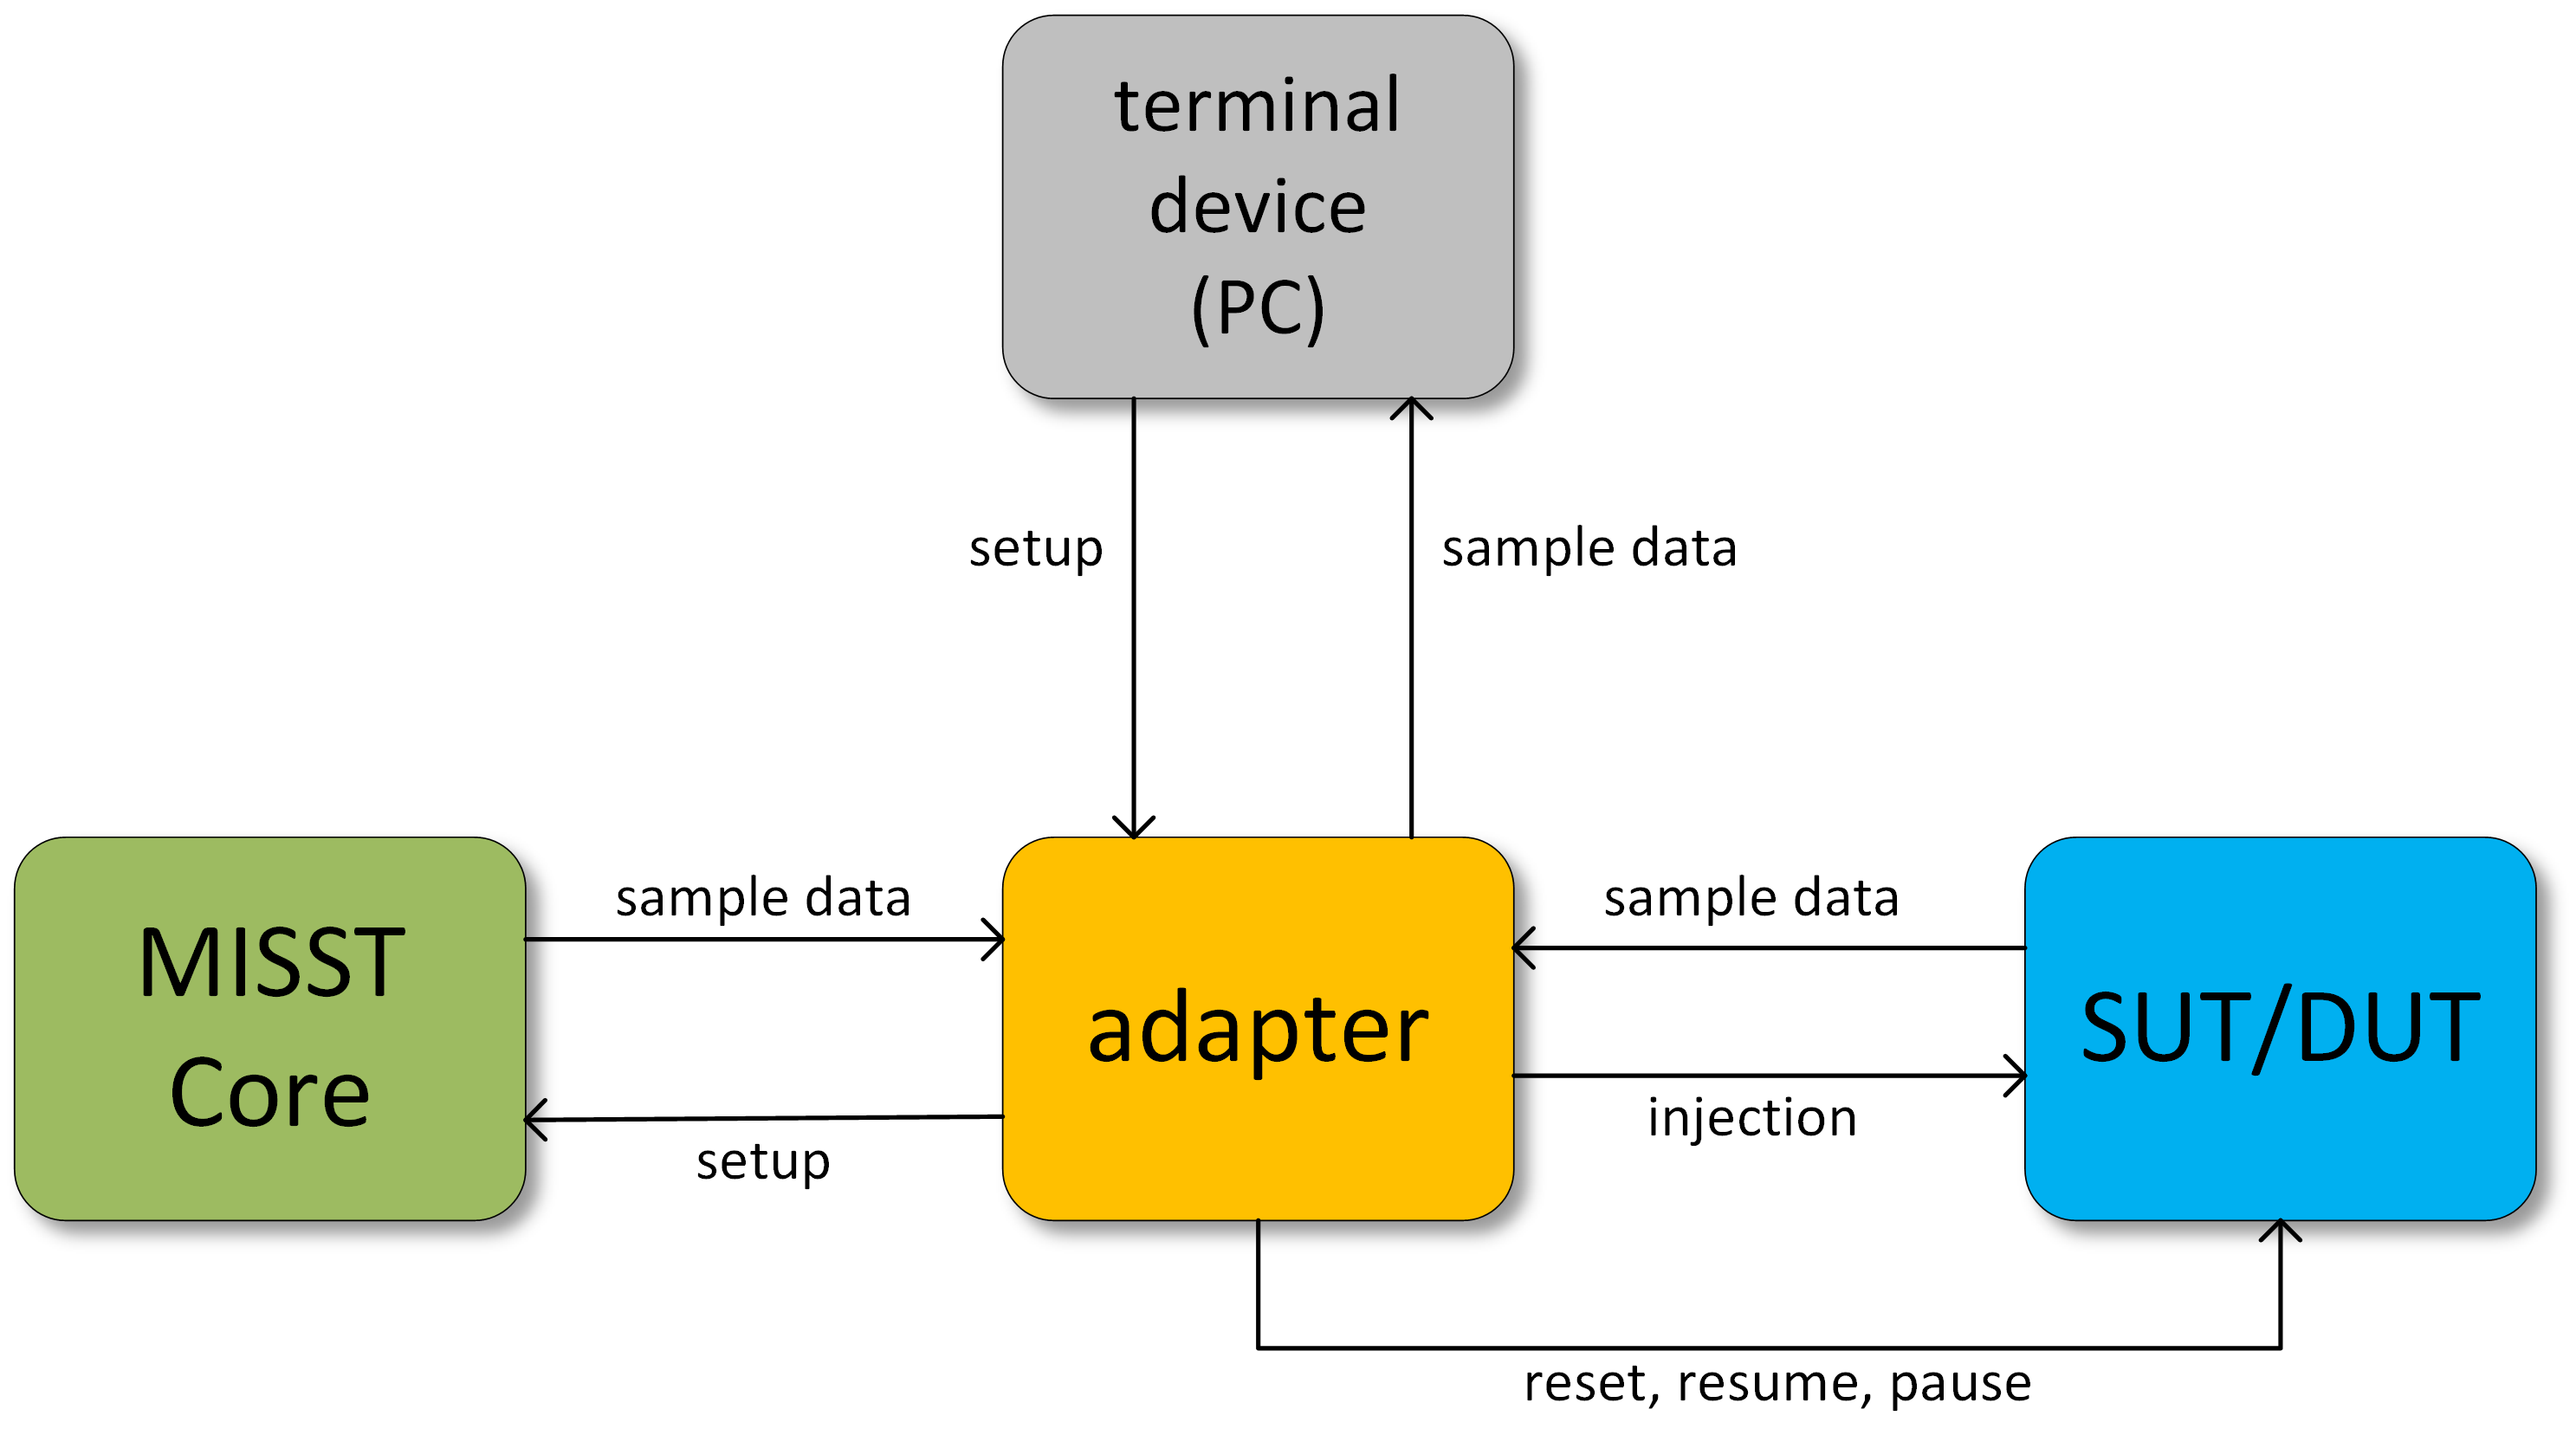
\includegraphics[width=0.7\linewidth]{../../technical_diags/f16_core_adapter_pc_dut_high_level}
	\caption{High Level View of a Use Case}
	\label{fig:high level use case}
\end{figure}

\FloatBarrier
%DONE
\section{Original Implementation}
\label{s orig imp}
The MISST was originally developed on a PYNQ-Z1 Digilent development board using Vivado Xilinx tools. The PYNQ-Z1 board contains a ZYNQ 7000 family IC with a Cortex-A9 processor integrated with an Artix-7 equivalent FPGA \cite{pynq board manual}. See chapter \ref{c original imp details} for PYNQ-Z1 board implementation details.


%=====================================================================
%DONE
\chapter{MISST Module Overview}
Overall system design schematics shown in Figure \ref{fig:high level application arch}. The MISST core and supplemental modules are implemented in the FPGA fabric, and the Cortex hard processor being outside of the fabric. The AXI slave interface is not part of the core system modules, but specific to the PYNQ implementation. However, how the AXI slave connects to the system core and its required functionality are part of a standard explained in \ref{s axi slave interface}. The AXI slave interface is an example of an adapter module used to communicate with the MISST system independent of implementation.

\begin{figure}[h]
	\centering
	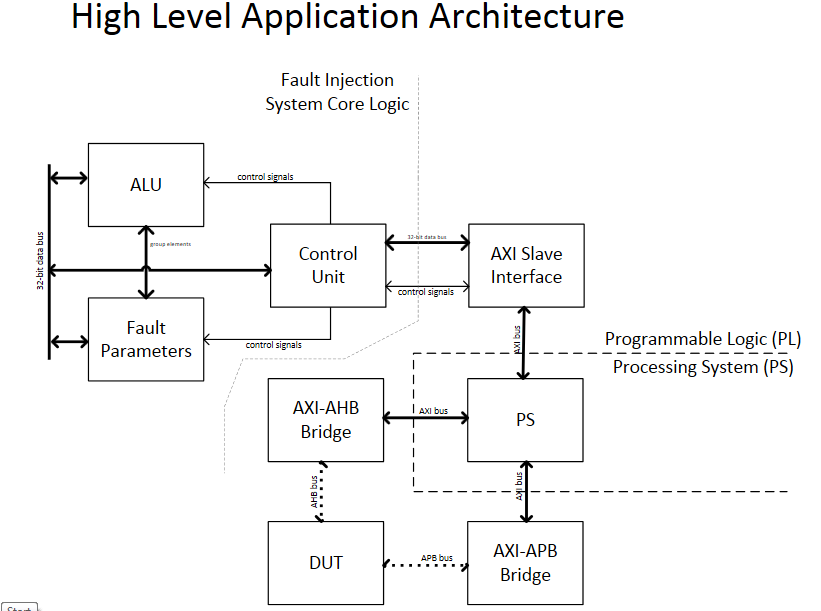
\includegraphics[width=0.7\linewidth]{../../technical_diags/f13_application_arch}
	\caption{High Level Implementation Architecture for Original Implementation}
	\label{fig:high level application arch}
\end{figure}

\clearpage

The MISST core logic is responsible for timing injections and sampling. It has three main modules: the Fault Parameters, an ALU, and the Control Unit. The Fault Parameters module is essentially memory holding information used to generate faults. The ALU is directly connected to the Fault Parameters module. The ALU is in charge of random number generation and changing the values saved in Fault Parameters. The Control Unit communicates with external modules and controls the ALU and Fault Parameter modules. The Control Unit is where MISST's basic behavior is implemented. Figure \ref{fig:core system interconnects} shows how the three modules are connected. 

\begin{figure}[h]
	\centering
	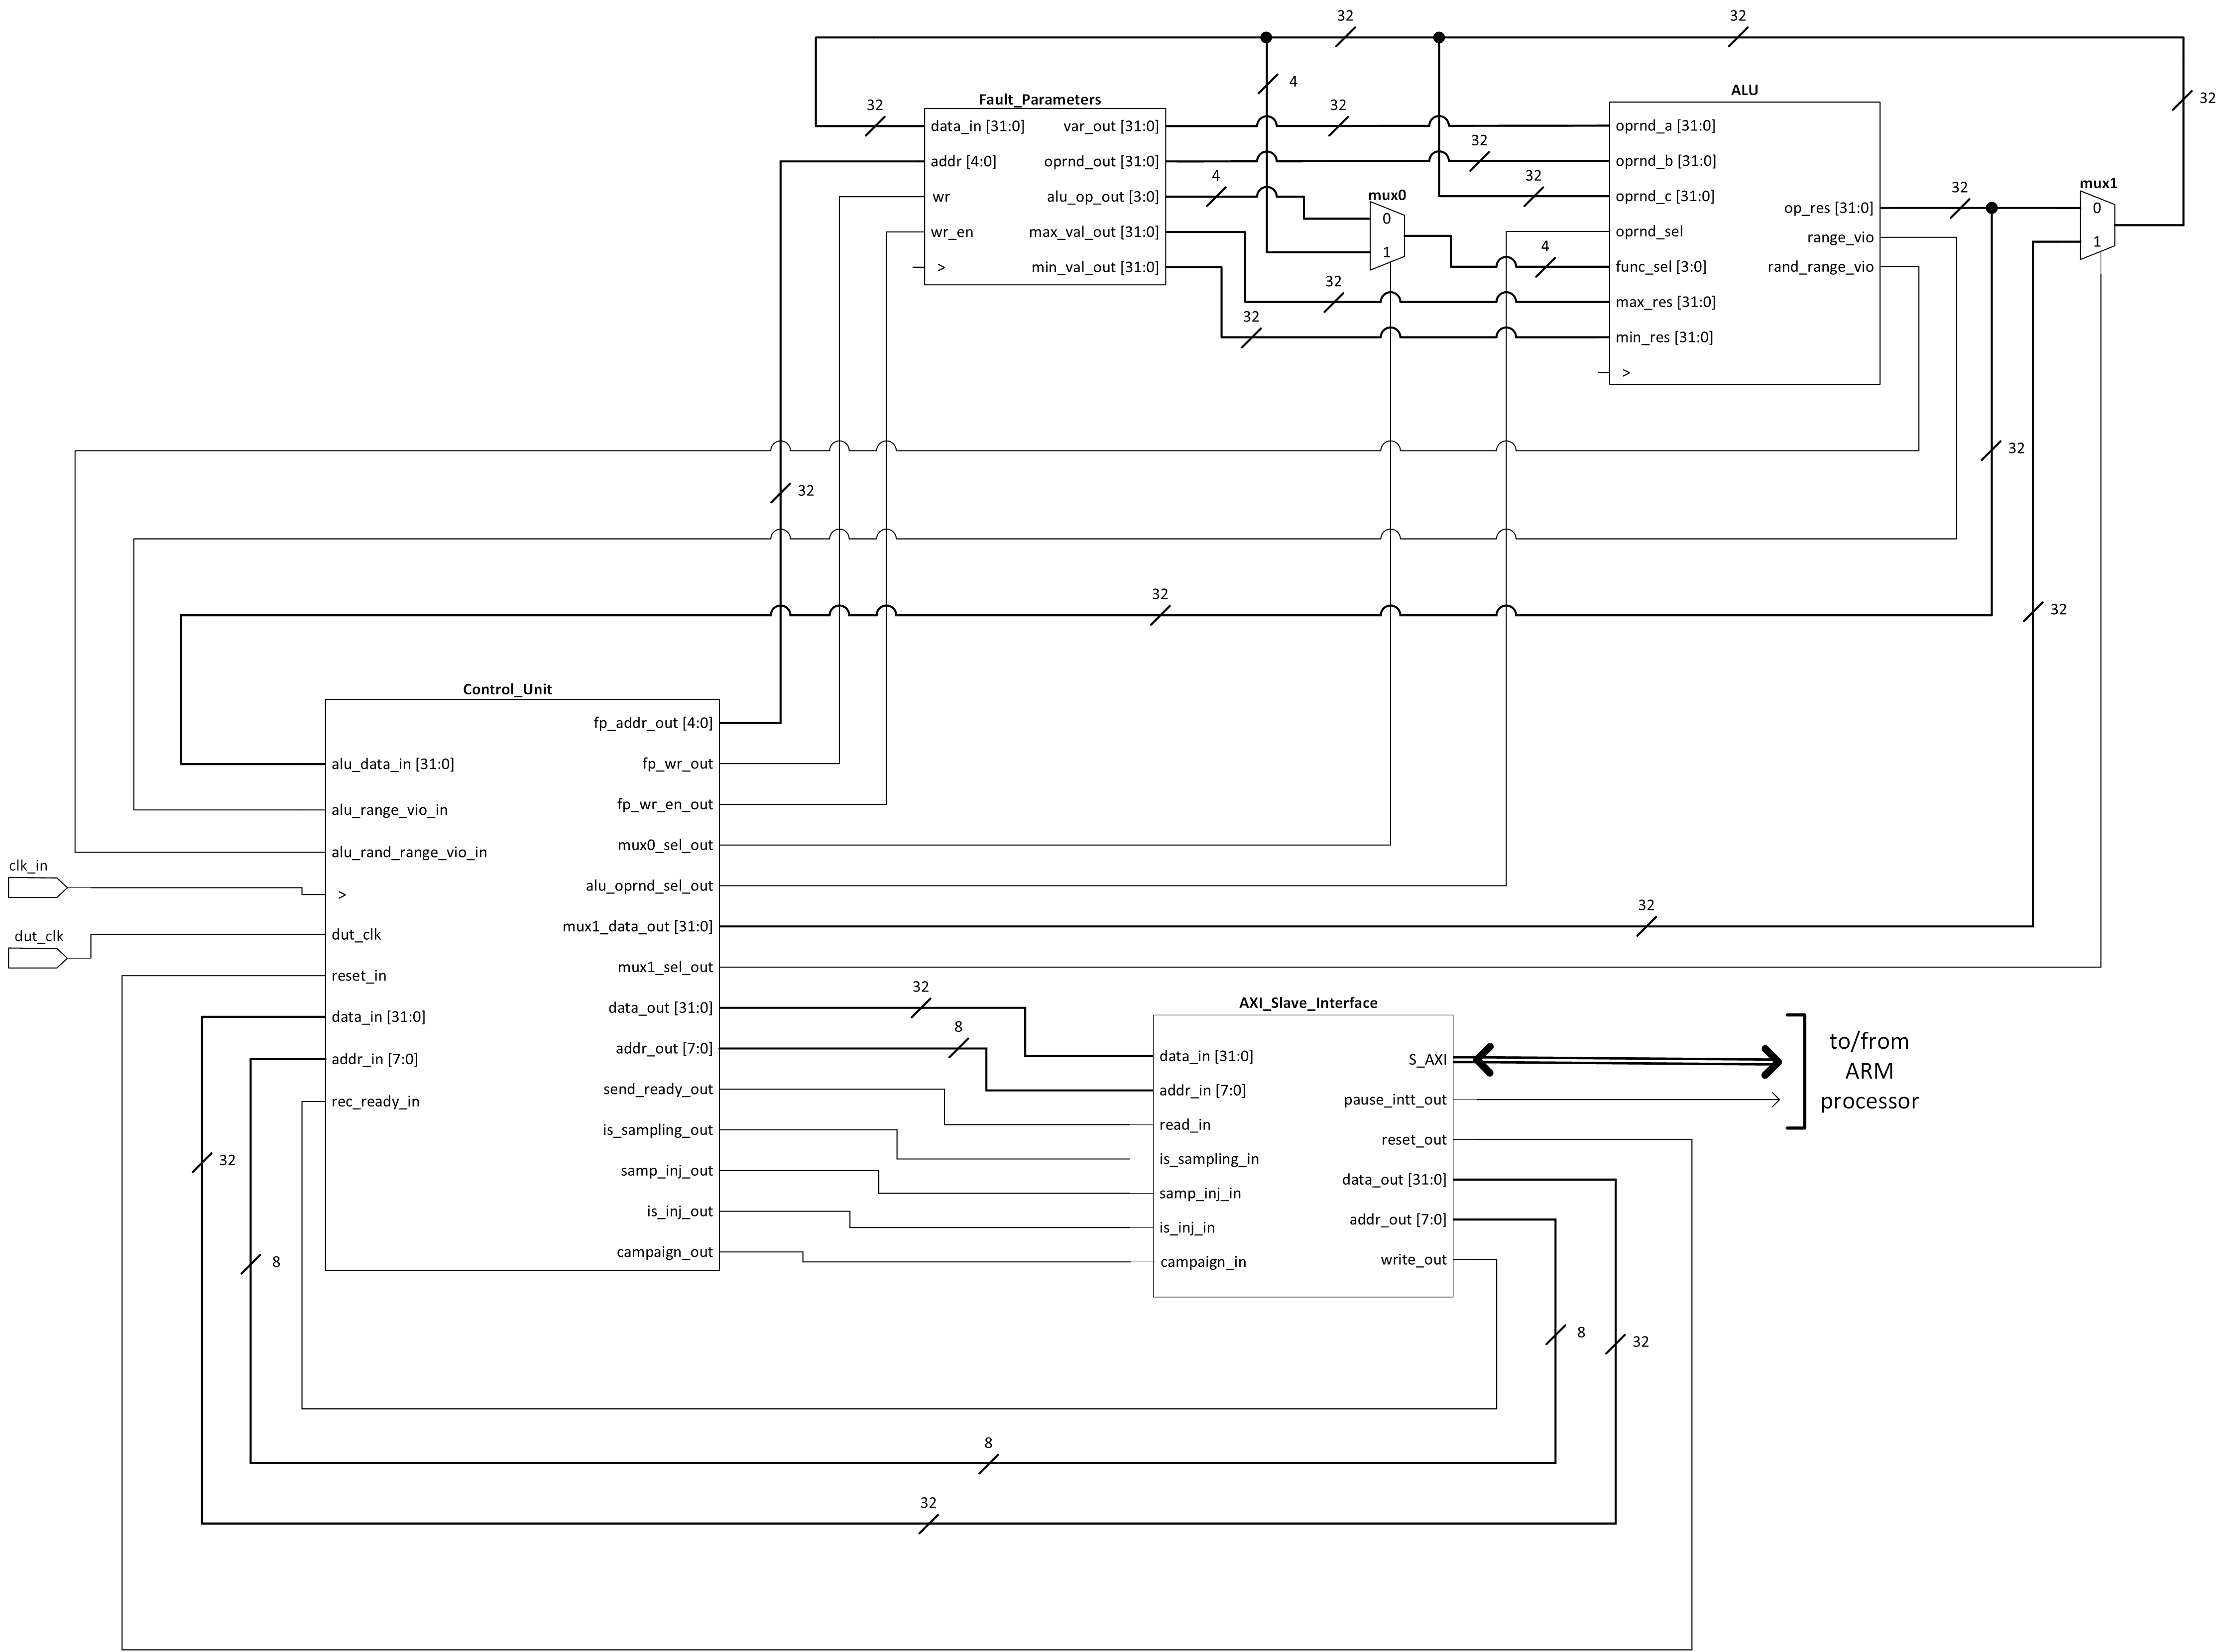
\includegraphics[width=0.7\linewidth]{../../visio_designs/overall_system_v2}
	\caption{MISST Core System Interconnect. The AXI Slave is not part of the core system.}
	\label{fig:core system interconnects}
\end{figure}

\clearpage
%DONE
\section{Task Flow}
\label{s task flow}

After the core and Adapter module have been implemented on an FPGA, the MISST system enters setup mode. In this state, the user can configure system registers listed in Table \ref{tab:register summary}. Once the user has configured MISST registers, the fault campaign begins. The general task flow for MISST is detailed in Figure \ref{fig:generaflowchart}. An injection or sample occurs when certain timers (see section \ref{s fault, samp, set timers}) timeout. If the injection and sampling timers timeout at the same time, sampling has priority. 

\begin{figure}[h]
	\centering
	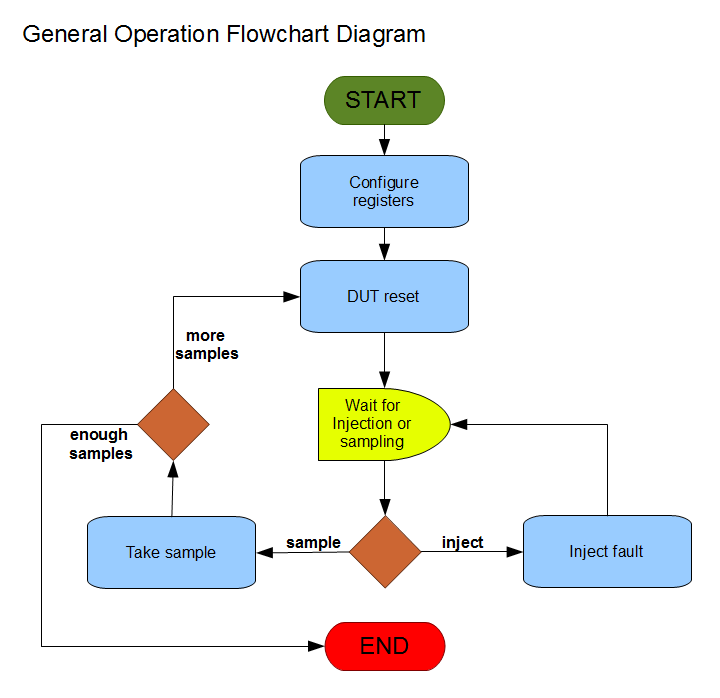
\includegraphics[width=0.7\linewidth]{../../technical_diags/f12_new_general_op_flowchart}
	\caption{General Task Flow for MISST}
	\label{fig:generaflowchart}
\end{figure}

\clearpage
%DONE
\subsection{Fault Generation}
\label{ss fault generation}

Injecting a fault involves three main steps:
\begin{enumerate}
	\item Retrieve DUT\_ADDR value from Fault Parameters module.
	\item Sample data at address DUT\_ADDR in the DUT memory space.
	\item Create fault data to inject from sampled data.
	\item Change fault parameters and save new INJ\_TIME value in fault\_timer register.
	\item Inject fault.
	\item Once acknowledgment from Adapter module has been received, resume the counters.
\end{enumerate}

In this section, step 5 will be explained. Every time a fault injection occurs, new parameters for the next injection are generated by using deterministic or random operations provided by the ALU. Fault parameters can change between every injection or change between a certain number of injections. Adding another layer of complexity, multiple fault parameters can be scheduled to change in different ways. For example, all three fault parameters can be configured to change for every fault request. Another possible scenario is that the dut\_addr fault parameter changes on every fault request and the flt\_oprnd changes every three times dut\_addr has been changed. When dut\_addr has been changed three times, it will revert to an initial value or 'initialized'. When a fault parameter changes, but not initialized, it has been 'updated'. In this example, flt\_oprnd would be on level 2, and dut\_addr on level 1.

Each fault parameter is assigned a level that represents how it changes. Level 2 fault parameters update every time an injection occurs. Level 1 fault parameters update every time level 2 fault parameters are initialized. Level 0 fault parameters update every time level 1 parameters are initialized. It is \textit{crucial} that if a level is meant to change throughout a fault campaign, that its lower levels (level 2 is the lowest level) are \textit{not} constants. 

A level's cycle length is the number of values in an initialize-update cycle. For example, a cycle length of 3 means that a fault parameter is initialized, updated, updated, and then the cycle is repeated again. A cycle length of two means that the fault parameter is initialized every other change. A cycle length of 1 means that the parameter does not change. A cycle length of 0 means that the parameter updates every time a fault generation is requested, like level 2. A cycle length of 0 should be used for randomly generated fault parameters.

%DONE
\subsubsection{Randomly Generated Injection Time}
\label{ss rand gen inj time}

Extra caution should be taken when injection time is configured to be generated randomly. Since injection time can't be predicted in advance, not all faults within a set can be injected before sampling occurs. \textit{All} faults in a set must be injected \textit{before} sampling to avoid injection and sampling at the same time. The MISST system doesn't explicitly enforce each set to have the same number of injects before sampling so the MISST system should be configured with that in mind. 

It's recommended that if injection time is randomly generated, sets be limited to only one fault. Configure the appropriate bounds for this injection time so that it occurs before sampling time. If multiple randomly generated injection time faults are desired, set the maximum value to the quotient of the sampling time and the number of injections per set. This should avoid any sampling or injection collisions.

%DONE
\subsubsection{Fault Generation Example}
\label{ss fault gen example}

To illustrate fault generation, we will provide the following example.

A MISST system is configured as follows:
\begin{itemize}
	\item Level 2 is dut\_addr parameter with a cycle length of 2. It is initialized to a value A\textsubscript{0}.
	\item Level 1 is flt\_oprnd parameter with a cycle length of 3 also. It is initialized to a value B\textsubscript{0}.
	\item Level 0 is inj\_time parameter with a cycle length of 1 so it stays constant at a value C.
\end{itemize}

As the fault parameters are changed during every injection process, the pattern in Figure \ref{fig:example fault gen timeline} emerges. In this example, the fifth fault would inject at address A\textsubscript{0} using value B\textsubscript{2} for flt\_oprnd, C clock cycles after the previous injection.  

\begin{figure}[h]
	\centering
	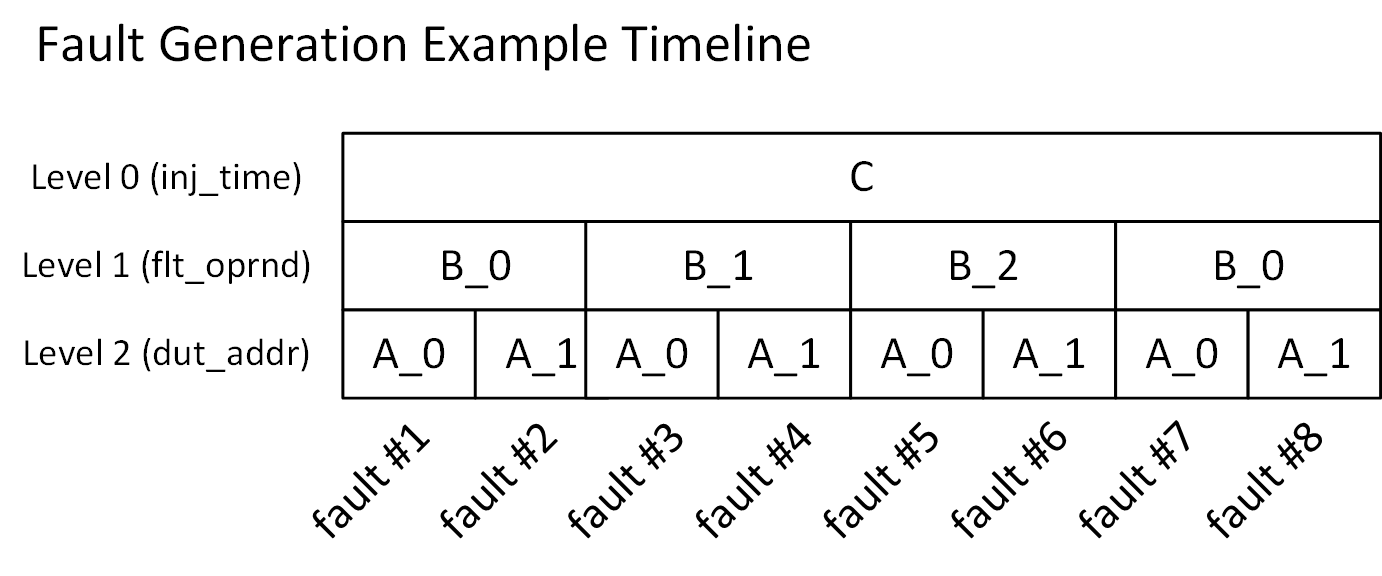
\includegraphics[width=0.7\linewidth]{../../technical_diags/f20_example_fault_gen_timeline}
	\caption{Fault Generation Example Timeline}
	\label{fig:example fault gen timeline}
\end{figure}

Actual test cases won't be as repetitive, and would involve longer cycle lengths. 

%DONE
\subsection{Fault Generation and Sampling Synchronization}

MISST considers a set to have completed after a successful sampling process initiated by the sampling timer timeout (see section \ref{s fault, samp, set timers}). MISST does not check if during a set any faults were injected, and does not enforce that each set have the same number of fault injections. Between DUT resets, the fault and sampling timer's count is reset to 0, but each timer's timeout value is left the same.

Generating faults in this manner allows the user flexibility to configure which faults are included within sets. Referring back to the example in section \ref{ss fault gen example}, if a user wants each set to have two faults so that the level 1 parameter changes after a sampling event, the user should set C (the inj\_time) no less than a third the sampling time and no more than half the sampling time. Another possibility is that each set contains three faults. In that case, faults 1 to 3 would be in the first set, faults 4 to 5 in the seconds, and so on.  

\clearpage
%DONE
\subsection{Sampling-based Shutdown}
\label{ss samping-based shutdown}

Sampling-based shutdown refers to ending a fault injection campaign based on the value of sampled data. If two locations are sampled, then the decision to shut down is based on the first sample. If MISST is configured to sample two locations, but sampling-based shutdown occurs, the second sample data will not be sent to the user. With the sampled value and the value in register sample\_shutdown\_value, there are three ways MISST evaluates sampling-based shutdown:
\begin{itemize}
	\item MISST shutdowns if sampled value equals sample\_shutdown\_value.
	\item MISST shutdowns if result of bitwise AND between sampled value and sample\_shutdown\_value is zero.
	\item MISST shutdowns if result of bitwise XOR between sampled value and sample\_shutdown\_value is zero.
\end{itemize}

%DONE
\section{Memory Organization}

MISST memory uses byte length addressing to write to different registers spread throughout the system core and the adapter module. There are three places where MISST addressable registers are implemented; in Fault Parameters, in Control Unit, and in the Adapter module. Table \ref{tab:register summary} explains each register's role in MISST. The address structure of Fault Parameters is different from the registers implemented in Control Unit and Adapter modules. See Section \ref{sec fp addr scheme} for more details on the Fault Parameter addresses. 

\begin{center}
	\begin{longtable}{| p{\linewidth} |}
		\caption{Complete Register Summary. \\ In the Read/Write column, 0 means used internally by system.}
		\label{tab:register summary}\\
		\hline 
		Address: Name Read/Write \newline Description\\ 
		\endfirsthead
		\caption{Complete Register Summary continued.}\\
		\hline
		Address: Name Read/Write \newline Description\\ 
		\endhead
		\hline 
		0x01  start\_inj  W  \newline 
		If the value 0xAABBCCDD is written to this register, a fault injection campaign will start. \\
		\hline 
		0x02  stop\_inj  W \newline 
		If the value 0xFFEEDDCC is written to this register, the fault injection campaign will stop.\\ 
		\hline 
		0x03  fault\_timer W \newline
		The number of clock cycles until a fault is injected into the DUT.\\ 
		\hline 
		0x04  sampling\_timer  W \newline 
		The time to sample after the last DUT reset measured in DUT clock cycles. \\ 
		\hline
		0x05  setNumCounter  W \newline 
		Maximum number of sets. This register is incremented after every sampling. Mainly used as a fail safe to stop MISST system after some failure has caused it to continue execution longer than expected.\\
		\hline
		0x06  triggerPosCU  W \newline 
		Holds trigger position inputs for cyc\_cnt modules. See Figure \ref{fig:control unit design} for reference.\\
		\hline
		0x07  dut\_addr\_init  W \newline 
		Initialization DUT\_ADDR value. The value that DUT\_ADDR is set to after an initialization event. In the case that the DUT\_ADDR fault parameter is constant, this register is unused.\\
		\hline
		0x08  inj\_time\_init  W \newline 
		Initialization INJ\_TIME value. The value that INJ\_TIME is set to after an initialization event. In the case that the INJ\_TIME fault parameter is constant, this register is unused.\\
		\hline
		0x09  flt\_oprnd\_init  W \newline 
		Initialization FLT\_OPRND value. The value that FLT\_OPRND is set to after an initialization event. In the case that the FLT\_OPRND fault parameter is constant, this register is unused.\\
		\hline 
		0x0A  sample\_dataA  0 \newline 
		Sampled data is saved here. \\ 
		\hline 
		0x0B  cont\_after\_inj  0 \newline 
		When 0x1F1F1F1F is written here, MISST is ready to continue after a fault injection.\\ 
		\hline 
		0x0C  sys\_status  R \newline 
		MISST system status. This register resides in the Adapter module (see chapter \ref{c adapter module}).
		\begin{itemize}
			\item bit 0: Set if system is executing an injection campaign, otherwise zero.
			\item bit 1: Set if system is sampling data that must be sent to user. Cleared after write to sample\_dataA register.
			\item bit 2: Set if system is sampling data that will not be sent to user. Cleared after write to sample\_dataA register.
			\item bit 3: Set if system requests a fault injection. Cleared after the correct value is written to cont\_after\_inj.
			\item bit 4: Set if DUT must be reset.
			\item bit 5: Set if two samples are taken. Otherwise zero.
			\item bit 6: Set if MISST is in setup mode.
			\item Other bits remain unused.
		\end{itemize}\\ 
		\hline 
		0x0D dut\_addr\_cyc\_len W \newline
		The cycle length of DUT\_ADDR. At the beginning of each cycle, DUT\_ADDR will be set to its initial value. A value of 1 means that DUT\_ADDR will never change. A value of 0 means that for every new fault generated, DUT\_ADDR will always be changed to a new value (this setting mainly used with random changes).\\
		\hline 
		0x0E inj\_time\_cyc\_len W \newline
		The cycle length of INJ\_TIME. At the beginning of each cycle, INJ\_TIME will be set to its initial value. A value of 1 means that INJ\_TIME will never change. A value of 0 means that for every new fault generated, INJ\_TIME will always be changed to a new value (this setting mainly used with random changes).\\
		\hline 
		0x0F flt\_oprnd\_cyc\_len W \newline
		The cycle length of FLT\_OPRND. At the beginning of each cycle, FLT\_OPRND will be set to its initial value. A value of 1 means that FLT\_OPRND will never change. A value of 0 means that for every new fault generated, FLT\_OPRND will always be changed to a new value (this setting mainly used with random changes).\\
		\hline
		0x10 sampling\_addrA W \newline
		Address to sample in DUT memory space. \\
		\hline
		0x11 sampling\_addrB W \newline
		Address to sample in DUT memory space. \\
		\hline
		0x12 general\_config W \newline
		General system configuration. Configures MISST high level behavior.
		\begin{itemize}
			\item bit[1:0] Selects fault parameter for Level 2. See (\ref{ss fault generation}) for level explanation. See Table \ref{table:fault char regs} for fault parameter values (the two least significant bits). 
			\item bit[3:2] Selects fault parameter for Level 1. See (\ref{ss fault generation}) for level explanation. See Table \ref{table:fault char regs} for fault parameter values (the two least significant bits).
			\item bit[5:4] Selects fault parameter for Level 0. See (\ref{ss fault generation}) for level explanation. See Table \ref{table:fault char regs} for fault parameter values (the two least significant bits).
			\item bit[6] If set, two locations will be sampled every time the sampling timer timeouts.
			\item bit[7] If set, MISST shutdowns if ALU experiences a non-random range violation during fault generation.
			\item bit[9:8] Determines how MISST will shutdown based on sample taken. If two samples are taken, the decision is based on first sample.
			\begin{itemize}
				\item b00 Shutdown is not based on sample value. 
				\item b01 MISST shutdowns if sample equals value stored in sample\_shutdown\_value register.  
				\item b10 MISST shutdowns if the resulting value of a bitwise AND between sample value and sample\_shutdown\_value register is 0. 
				\item b11 MISST shutdowns in a similar fashion as the previous, but with a bitwise XOR operation.
			\end{itemize}
		\end{itemize}\\
		\hline
		0x13 sample\_shutdown\_value W \newline
		Value used for sample based shutdown. \\
		\hline
		0xC0 dut\_sample\_addr 0 \newline
		Address to be sampled. This is implemented in the Adapter module. See Table \ref{table:axi slave int regs}. \\
		\hline
		0xC1 dut\_inj\_addr 0 \newline
		Address of injection. This is implemented in the Adapter module. See Table \ref{table:axi slave int regs}.\\
		\hline
		0xC2 dut\_data\_out 0 \newline
		Data to be written to DUT. This is implemented in the Adapter module. See Table \ref{table:axi slave int regs}.\\
		\hline
		0xC3 w\_reg\_addr W \newline
		MISST register address. This is implemented in the Adapter module. See Table \ref{table:axi slave int regs}.\\
		\hline
		0xC4 w\_data W \newline
		Write data for MISST core. This is implemented in the Adapter module. See Table \ref{table:axi slave int regs}.\\
		\hline
	\end{longtable} 
\end{center}

%=====================================================================
%DONE
\chapter{Fault Parameters Module}
\label{c fp module}

The main role of this module is to store the fault parameters, and provide associated data to the ALU for fault generation (see section \ref{ss fault generation}). There are three fault parameters and they are listed in Table \ref{table:fault char regs}. How fault parameters affect a set of faults is shown by Figure \ref{fig:case characteristics}.

\begin{figure}[h]
	\centering
	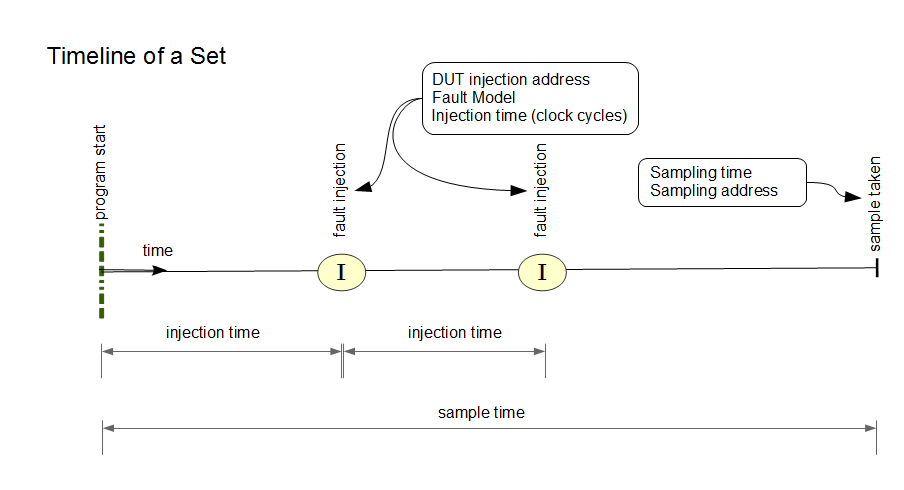
\includegraphics[width=0.9\linewidth]{../../technical_diags/f22_timeline_of_set}
	\caption{Fault Parameters on Set Timeline}
	\label{fig:case characteristics}
\end{figure}

\clearpage
%DONE
\section{Structure}

The Fault Parameters module is a collection of three submodules (one for each fault parameter) called a grouping. Each grouping contains five registers related to the fault parameter referred to as an element. Table \ref{table:fault char regs} explains each fault parameter, and Table \ref{table:element summary} describes each element in a grouping. Figure \ref{fig:fp structure} details how groupings are connected.
\begin{figure}[h]
	\centering
	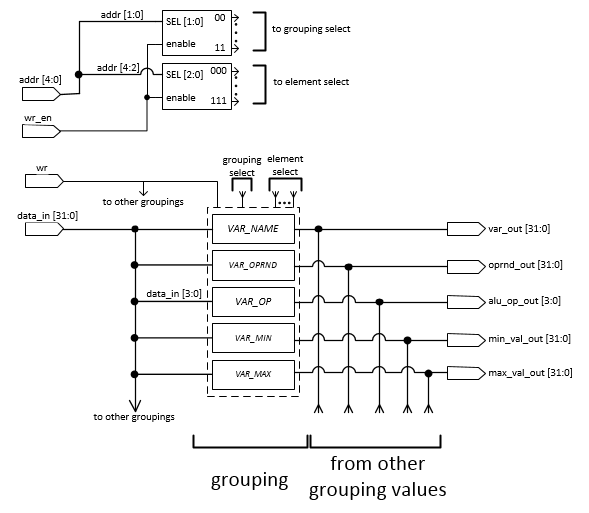
\includegraphics[width=0.75\linewidth]{../../technical_diags/f5_planned_vr_interconnect}
	\caption{Fault Parameters Structure}
	\label{fig:fp structure}
\end{figure}

\clearpage
%DONE
\section{Address Scheme}
\label{sec fp addr scheme}
When the three most significant bits are b100, the address refers to memory in the Fault Parameters. The address has two parts: the two least significant bits refer to a fault parameter, and the next three bits refer to a fault parameter element. Tables \ref{table:fault char regs} and \ref{table:element summary} explain the possible addresses.

\begin{table}[h]
	\centering
	\caption{Fault Characteristic Registers. The 'X' denote "don't cares".}
	\begin{tabular}{|c|c|p{9cm}|}
		\hline 
		Address & Name & Description \\ 
		\hline 
		0b100X-XX00 & DUT\_ADDR & Current value of injection address in DUT memory space. \\ 
		\hline 
		0b100X-XX01 & INJ\_TIME & Current value of injection time. Injection time is measured as the number of DUT clock cycles since the previous fault injection or DUT reset if this will be first fault in a set.  \\ 
		\hline 
		0b100X-XX10 & FLT\_OPRND & Short for fault operand. Depends on type of fault. For a SEU, it's the bit mask of bits to invert. For additive error model, it's the additive error. \\ 
		\hline 
	\end{tabular} 
	\label{table:fault char regs}
\end{table}

\begin{table}[h]
	\centering
	\caption{Fault Parameter Element Summary. The 'X' denote "don't cares".}
	\begin{tabular}{|c|c|p{9cm}|}
		\hline 
		Address & Suffix & Description \\ 
		\hline
		0b1000-00XX & \_NAME & Value of associated fault parameter.\\
		\hline
		0b1000-01XX & \_OPRND & Operand for arithmetic operation used when changing the value of the fault parameter. \\ 
		\hline 
		0b1000-10XX & \_OP & Arithmetic operation to change fault parameter. Unlike the other elements which are 4 bytes, this element is a nibble. NOP (no operation) function denotes a constant fault parameter. \\ 
		\hline 
		0b1000-11XX & \_MIN & Minimum possible value of fault parameter, inclusive. \\ 
		\hline 
		0b1001-00XX & \_MAX & Maximum possible value of fault parameter, inclusive. \\ 
		\hline 
	\end{tabular} 
	\label{table:element summary}
\end{table}
\clearpage
%DONE
\section{Port Descriptions}
\label{s fp port summ}

\begin{table}[th]
	\centering
	\caption{Fault Parameters Port Descriptions}
	\label{table:fp port desc}
	\begin{tabular}{|c|p{0.7\textwidth}|}
		\hline 
		Port Name & Description \\ 
		\hline 
		data\_in [31:0] & Write input data bus.\\  
		\hline
		addr [4:0]& Address input bus. Addresses explained in section \ref{sec fp addr scheme}.\\
		\hline
		wr\_en & A chip enable. Must be high for element values to output.\\
		\hline
		wr & Write enable on rising edge.\\
		\hline
		var\_out [31:0] & NAME element for currently selected grouping.\\
		\hline
		oprnd\_out [31:0] & OPRND element for currently selected grouping.\\
		\hline
		alu\_op\_out [3:0] & OP element for currently selected grouping.\\
		\hline
		min\_val\_out [31:0] & MIN element for currently selected grouping.\\
		\hline
		max\_val\_out [31:0] & MAX element for currently selected grouping.\\
		\hline
	\end{tabular}
\end{table}

%=====================================================================
%DONE
\chapter{The ALU}
\label{c: the alu}

%DONE
\section{Mathematical Operations}
The ALU changes fault parameters based on a fault parameter's elements. Other than providing common arithmetic operations, the ALU provides random number generation. The operation is chosen through the func\_sel input port as a nibble. These values are shown in Table \ref{table: alu op-codes}.
\begin{table}[h]
	\centering
	\caption{ALU Op-Codes}
	\label{table: alu op-codes}
	\begin{tabular}{|c|c|l|}
		\hline 
		Code & Operation & Result \\ 
		\hline 
		0x0 & no operation & Outputs input to oprnd\_a port. \\
		\hline
		0x1 & addition & The sum of oprnd\_a and selected second operand. \\
		\hline
		0x2 & increment & The value of oprnd\_a incremented by one. \\
		\hline
		0x3 & decrement & The value of oprnd\_a decremented by one. \\
		\hline
		0x4 & left shift & Single left shift of oprnd\_a. \\
		\hline
		0x5 & right shift & Single right shift of oprnd\_a. \\
		\hline
		0x6 & OR & Bitwise OR of oprnd\_a and selected second operand.\\
		\hline
		0x7 & AND & Bitwise AND of oprnd\_a and selected second operand.\\
		\hline
		0x8 & subtraction & Difference between oprnd\_a and selected second operand.\\
		\hline
		0x9 & unimodal Gaussian & A random number with a unimodal, Gaussian distribution.\\
		\hline
		0xA & uniform uniform & A random number with a uniform distribution with no variance.\\
		\hline
		0xB & uniform average & A random number with a uniform distribution with some variance. \\
		\hline
		0xC & bimodal Gaussian & A random number with a bimodal, Gaussian distribution.\\
		\hline
		0xD & random bit flip & Inverts a single, randomly selected bit in the least significant byte of oprnd\_a.\\
		\hline 
	\end{tabular} 
\end{table}

\clearpage
%DONE
\section{Random Number Generation}

The ALU contains a module called noise\_gen to generate random numbers with specified distributions. The VHDL source code for this module is originally from \cite{noise gen site}. The noise\_gen module generates random values using linear feedback shift registers. The four possible distributions generated are shown in Figure \ref{fig:noise gen distributions} for 16-bit random numbers.

The noise\_gen module has two outputs, Gaussian and uniform, that produce random numbers. Each of these outputs have two subtypes. To produce all four possible distributions, the ALU has two noise\_gen modules. However, at the moment they produce 16-bit numbers. Unfortunately, noise\_gen is not scalable because of the properties of linear feedback shift registers.  

\begin{figure}[h]
	\centering
	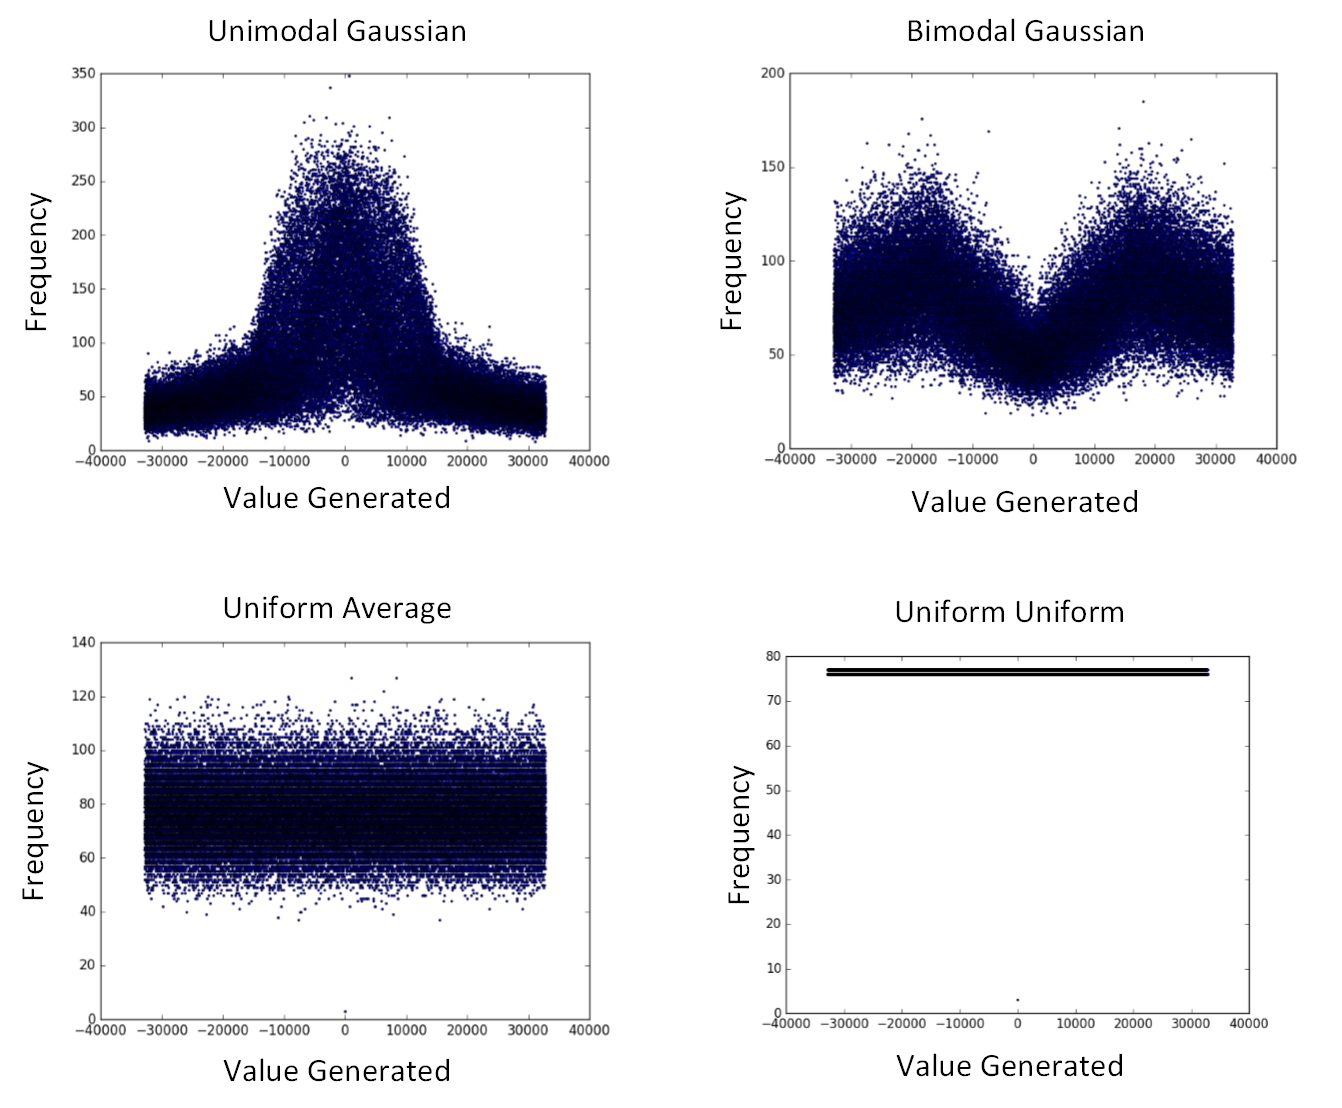
\includegraphics[width=0.95\linewidth]{../../technical_diags/f21_noise_gen_distributions}
	\caption{Distribution Tests for 16-bit Random Number Generation}
	\label{fig:noise gen distributions}
\end{figure}

%DONE
\section{Port Descriptions}

\begin{table}[h]
	\centering
	\caption{ALU Port Descriptions}
	\label{table:alu port desc}
	\begin{tabular}{|c|p{0.7\textwidth}|}
		\hline 
		Port Name & Description \\ 
		\hline 
		oprnd\_a\_in [31:0] & Operand A. This operand is used in single operand operations.\\
		\hline
		oprnd\_b\_in [31:0] & Operand B.\\
		\hline
		oprnd\_c\_in [31:0] & Operand C. The optional operand selected by setting oprnd\_sel\_in.\\
		\hline
		min\_res\_in [31:0] & Lower bound (inclusive) for ALU result.\\
		\hline
		max\_res\_in [31:0] & Upper bound (inclusive) for ALU result.\\
		\hline
		func\_sel\_in [3:0] & Selects ALU operation. See Table \ref{table: alu op-codes} for op-codes.\\
		\hline
		oprnd\_sel\_in & If set, oprnd\_c\_in is the second operand, otherwise the second operand is oprnd\_b\_in.\\
		\hline
		clk\_in & Clock input.\\
		\hline
		range\_vio\_out & Set if ALU result for a non-random operation is not between the values of min\_res\_in and max\_res\_in.\\
		\hline
		rand\_range\_vio\_out & Set if ALU result for a random operation is not between the values of min\_res\_in and max\_res\_in.\\
		\hline
		op\_res\_out [31:0] & Result of selected operation.\\
		\hline
	\end{tabular}
\end{table}

%=====================================================================
%DONE
\chapter{The Control Unit}

The Control Unit is responsible for MISST high level behavior. This includes:
\begin{itemize}
	\item Fault parameter generation.
	\item Sampling scheduling.
	\item Injection scheduling.
	\item External communication via Adapter module.
	\item Writing to registers.
\end{itemize}

%DONE
\section{Structure}
\label{s cu structure}
To carry out the aforementioned tasks, the Control Unit is implemented using three modules; the register control, the memory interconnect, and the injection campaign finite state machine (ICF). These modules and their interconnections are detailed in Figure \ref{fig:control unit design}. Note that registers are represented as rectangles labeled with the register's name. All these registers are implemented in the memory interconnect submodule. Figure \ref{fig:control unit design} also shows three cycle counter modules (labeled cyc\_cnt\#). Cycle counter modules count cycles of a signal and are further explained in section \ref{ss cyc cnt}. Cycle counter 0 counts DUT clock cycles until a fault injection occurs. Cycle counter 1 counts DUT clock cycles until a sampling event occurs. Cycle counter 2 counts the number of sets (essentially the number of sample events) until the maximum number of sets to shut down. 

\clearpage
\begin{figure}[h]
	\centering
	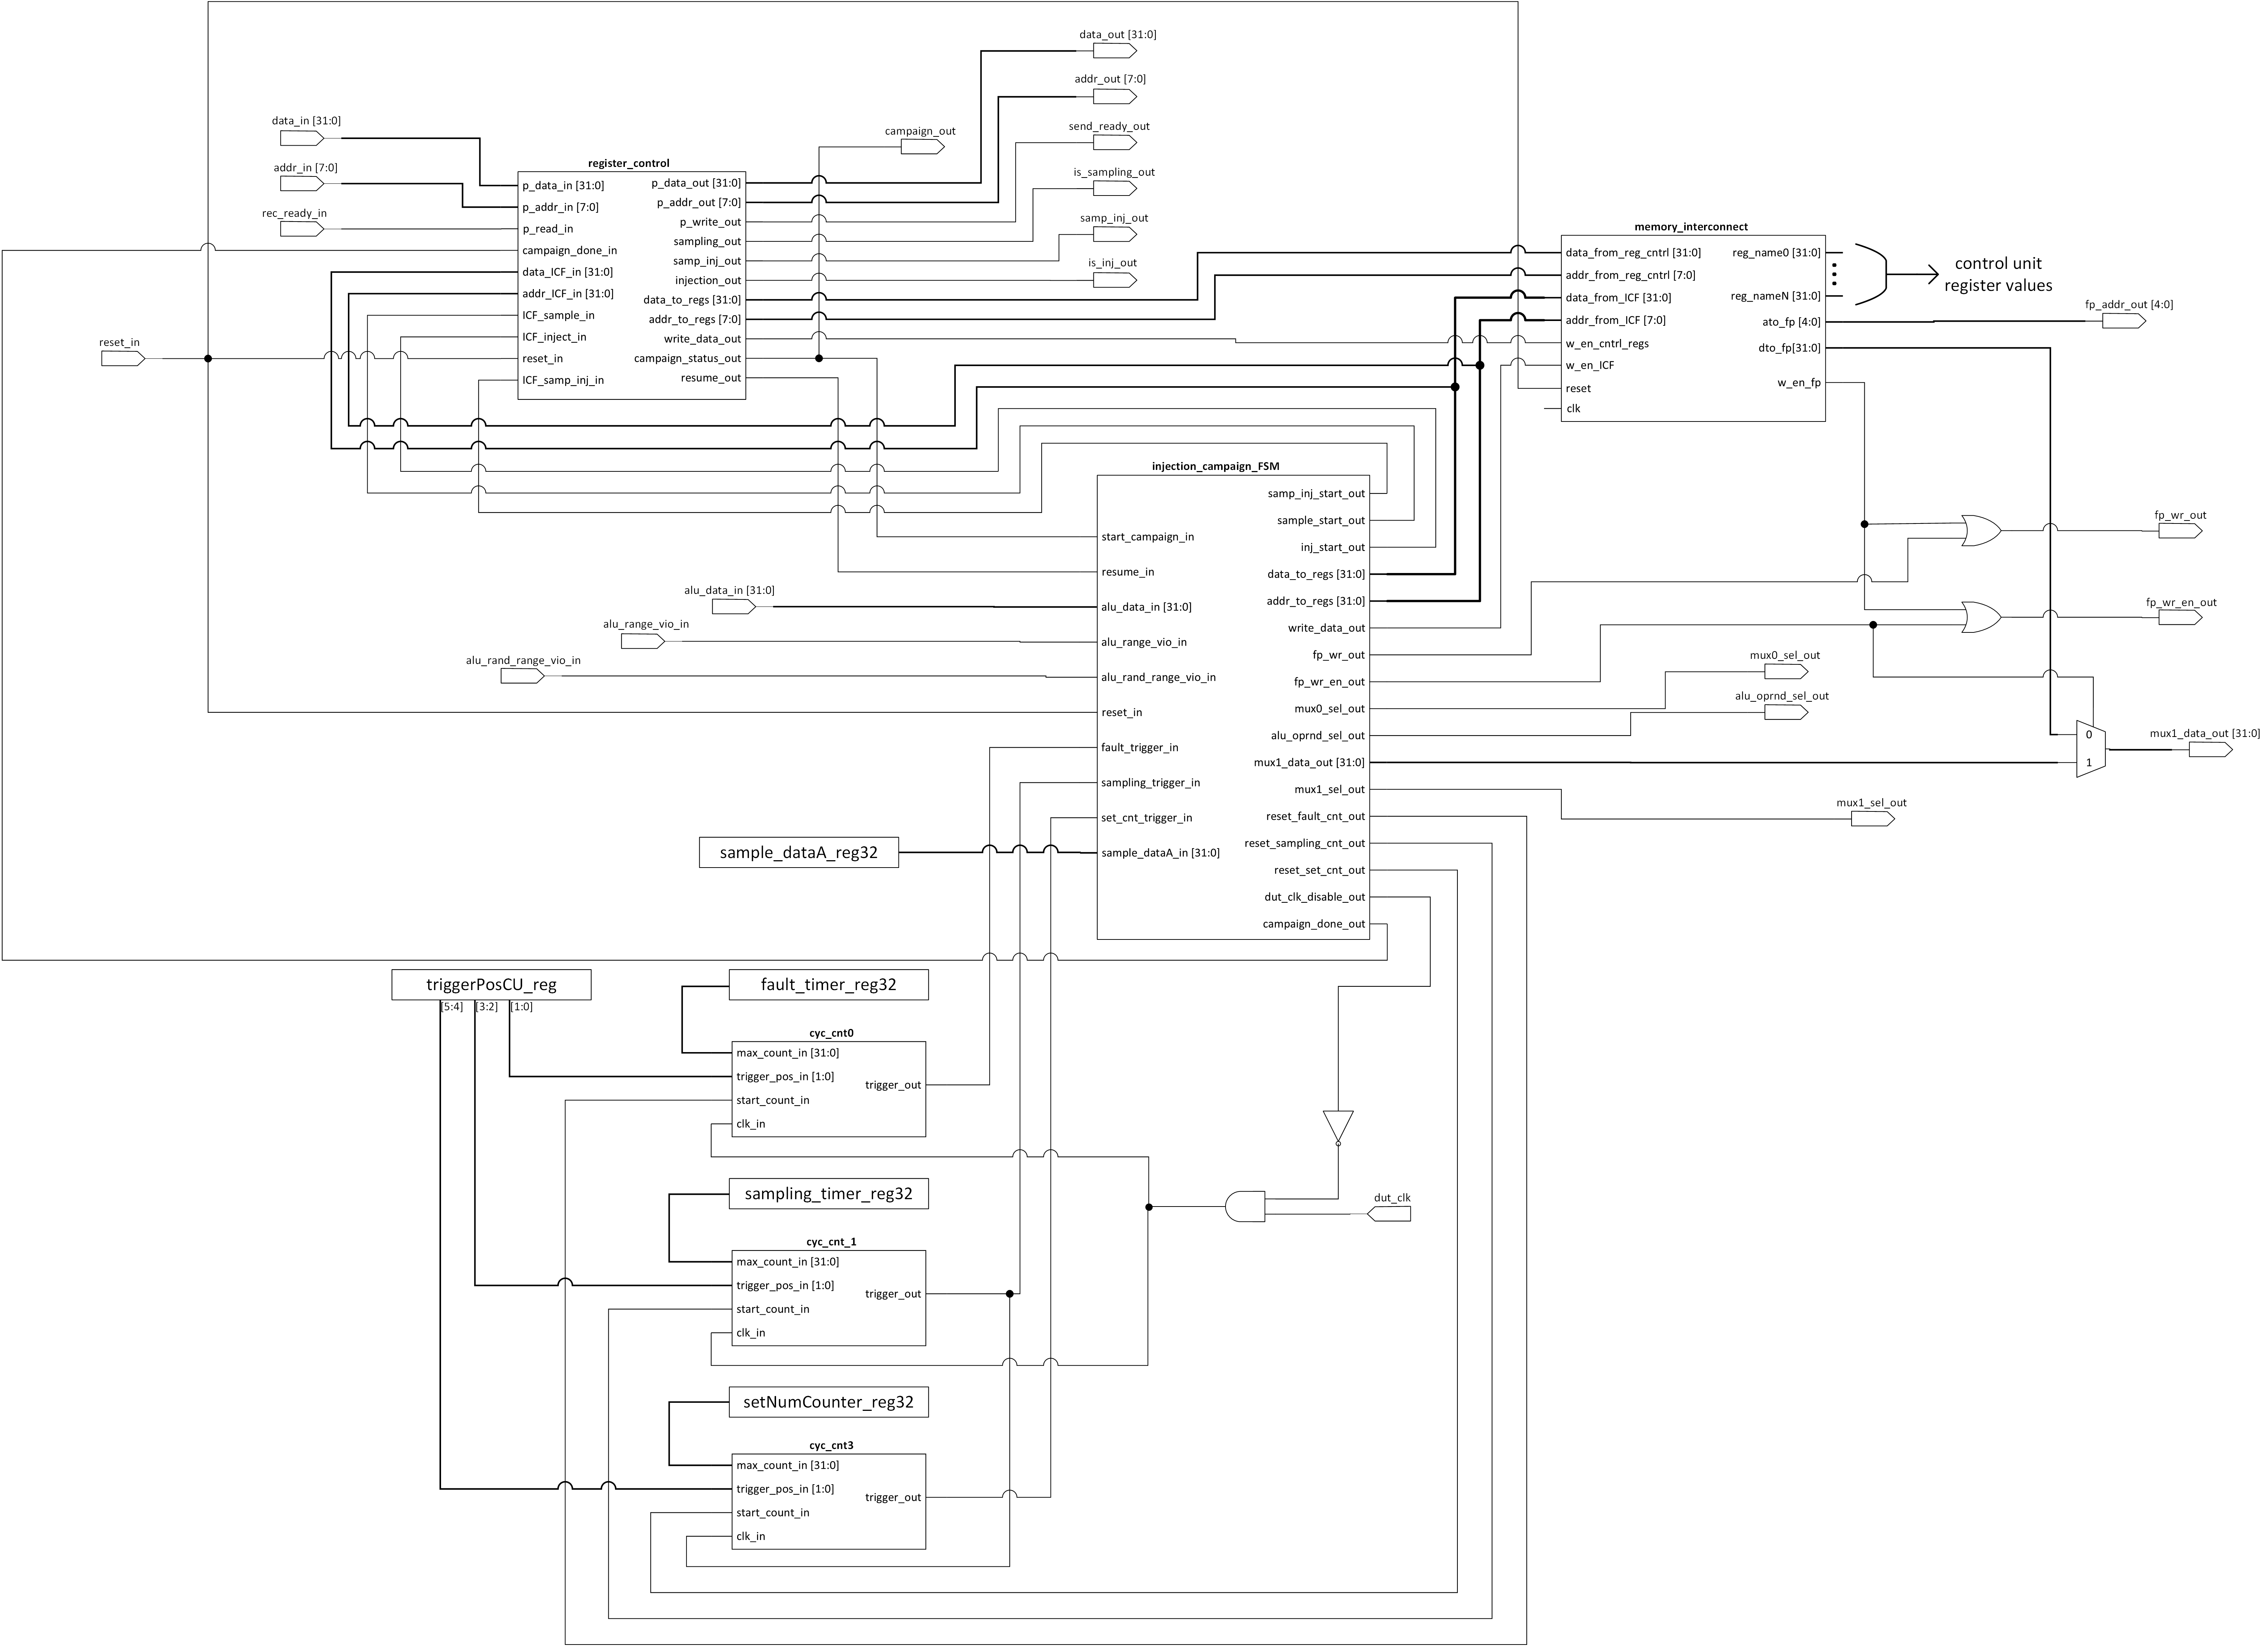
\includegraphics[width=1.0\linewidth]{../../visio_designs/Control_Unit_design}
	\caption{Control Unit Implementation}
	\label{fig:control unit design}
\end{figure}

\clearpage
%DONE
\subsection{Cycle Counter Module}
\label{ss cyc cnt}

The cycle counter module is especially designed for use in MISST. The cycle counter module simply counts rising edges of the input signal on clk\_in port until the number of rising edges hits a given value. Table \ref{table: cyc cnt ports} explains the role of each port.

\begin{table}[h]
	\centering
	\caption{Cycle Counter Ports}
	\label{table: cyc cnt ports}
	\begin{tabular}{|c|c|p{10cm}|}
		\hline 
		Port & Polarity & Description \\ 
		\hline 
		max\_count\_in [31:0] & input & Maximum number of cycles to count.\\ 
		\hline 
		trigger\_pos\_in [1:0] & input &  When the counter hits the maximum cycle count, this value determines on which edge of clk\_in the port trigger\_out asserts. See Figure \ref{fig:cyclecounterplot} for a timing diagram.
		\begin{itemize}
			\item b00 trigger\_out asserts on first rising edge (aka front edge) of clk\_in.
			\item b01 trigger\_out asserts on first falling edge (aka middle edge) of clk\_in.
			\item b10 trigger\_out asserts on last rising edge (aka back edge) of clk\_in. This option essentially delays trigger\_out by one clock cycle.
			\item b11 trigger\_out never asserts
		\end{itemize} \\ 
		\hline 
		start\_count\_in & input & Resets count to zero.\\ 
		\hline 
		clk\_in & input &  A rising edge increments count. Named clk\_in because this module is generally used to count clock cycles. \\ 
		\hline 
		trigger\_out & output & A rising edge indicates that the number of counts exceeds the value of man\_count\_in.\\ 
		\hline 
	\end{tabular} 
\end{table}

The trigger\_pos\_in port controls on which edge of the clk\_in signal the trigger\_out port will assert. Figure \ref{fig:cyclecounterplot} shows the timing diagram of a counter with a max count value of three. Note that the start\_cnt\_in input doesn't have to be kept high, but in this instance it is. The cycle counter multiplexes between the three internal signals front\_edge\_s, back\_edge\_s, and middle\_edge\_s for the trigger\_out output. All three signals assert during the third cycle of clk\_in, but they differ during which edge of that cycle they assert. For example, middle\_edge\_s asserts on the middle edge (the falling edge) of the third cycle of clk\_in.

\begin{figure}[h]
	\centering
	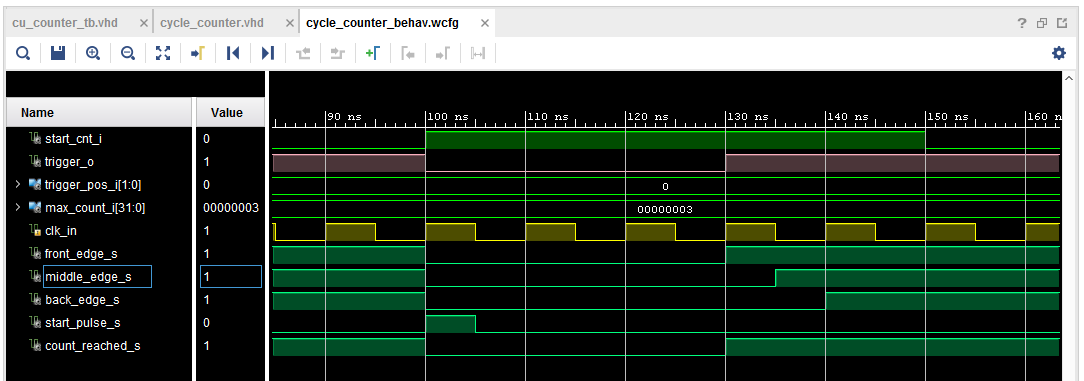
\includegraphics[width=0.95\linewidth]{../../technical_diags/c10_cycle_counter_sim_centered_start}
	\caption{Different Types of Trigger Position}
	\label{fig:cyclecounterplot}
\end{figure}


%DONE
\subsection{Register Control}
\label{ss reg control}

The register control module is responsible for processing incoming and outgoing data between the MISST core and the Adapter module.  Table \ref{table:reg control port desc} describes the ports of the register control module.

The register control module receives data from the Adapter module and forwards it to the memory interconnect. Register control also receives data from the ICF module (see section \ref{ss icf}) for fault injection and sampling. Note than in Table \ref{table:reg control port desc} the module distinguishes between two types of sampling: sampling data to corrupt and use in upcoming fault injection (sample inject), and sampling data to send to user (simply referred to as sampling). 

\begin{center}
	\begin{longtable}{|c|p{11cm}|}
		\caption{Register Control Port Descriptions}
		\label{table:reg control port desc}\\
		\hline 
		Port Name & Description \\ 
		\hline 
		\endfirsthead
		\caption{Register Control Port Descriptions Continued}\\
		\hline
		Port Name & Description\\
		\endhead
		\hline
		p\_data\_in [31:0] & Data bus for incoming data to MISST core. Part of the Adapter-Core Interface (see section \ref{s axi slave interface}). \\ 
		\hline 
		p\_addr\_in [7:0] &  Address bus for incoming data to MISST core. Part of the Adapter-Core Interface (see section \ref{s axi slave interface}).\\ 
		\hline 
		p\_read\_in & A logic high during a rising edge of clk\_in initiates a read of address and data buses from Adapter module (see section \ref{s axi slave interface}).\\ 
		\hline 
		campaign\_done\_in & Rising edge signals end of fault campaign. \\ 
		\hline 
		data\_ICF\_in [31:0] & Data from the ICF module (see section \ref{ss icf}) to be sent to Adapter module. \\ 
		\hline 
		addr\_ICF\_in [31:0] & Address in DUT address space for injection or sampling from the ICF module (see section \ref{ss icf}) to be sent to Adapter module. \\ 
		\hline 
		ICF\_sample\_in & Initiates a sampling operation on a rising edge. Sampled data is sent to the user via the Adapter module.\\
		\hline
		ICF\_samp\_inj\_in & Initiates a sampling operation on a rising edge. Sampled data is not sent to the user. This port used when retrieved data for a fault injection.\\
		\hline
		ICF\_inject\_in & Initiates a fault injection on the rising edge.\\
		\hline
		clk\_in & Clock input.\\
		\hline
		reset\_in & Initializes registers to zero on rising edge.\\
		\hline
		p\_data\_out [31:0] & Data bus for outgoing data to MISST core. Part of the Adapter-Core Interface (see section \ref{s axi slave interface}).\\
		\hline
		p\_addr\_out [7:0] & Address bus for outgoing data to MISST core. Part of the Adapter-Core Interface (see section \ref{s axi slave interface}).\\
		\hline
		p\_write\_out & A logic high during a rising edge of clk\_in initiates a write of address and data buses to Adapter module (see section \ref{s axi slave interface}).\\
		\hline
		data\_to\_regs\_out [31:0] & Data bus to memory interconnect module.\\
		\hline
		addr\_to\_regs\_out [7:0] & Address bus to memory interconnect module.\\
		\hline
		write\_data\_out & Rising edge enables write to MISST registers.\\
		\hline
		campaign\_status\_out & High during a fault injection campaign, and low when MISST is idle or during setup.\\
		\hline
		sampling\_out & A high value signals that sampling is in progress and that MISST is waiting for incoming data. Part of the Adapter-Core Interface (see section \ref{c adapter module}). Cleared when sampling data received.\\
		\hline
		samp\_inj\_out & A high value signals that sampling (specifically for retrieving data in preparation for a fault injection) is in progress and that MISST is waiting for incoming data. Part of the Adapter-Core Interface (see section \ref{c adapter module}). Cleared when sampling data received.\\
		\hline
		injection\_out & A high value signals that MISST is in the process of injecting a fault and that MISST is waiting for incoming data. Part of the Adapter-Core Interface (see section \ref{c adapter module}). Cleared when the cont\_after\_inj register is written with proper value signaling injection process completion and DUT execution resume (see section \ref{tab:register summary}).\\
		\hline
		resume\_out & A rising edge signals that MISST can resume execution after sampling (for user data or for injection data), DUT reset, or fault injection.\\
		\hline
	\end{longtable} 
\end{center}

%DONE
\subsection{Memory Interconnect}
\label{ss mem interconnect}

The memory interconnect module has two roles: implement Control Unit registers, and pass on Fault Parameter data. The memory interconnect module receives data from the register control and ICF modules. If a write to the same address at the same time occurs, the data from the ICF takes precedence. Table \ref{table:mem inter port desc} describes the ports of the memory interconnect module, but the register outputs are excluded. The only registers not implemented in the memory interconnect module are listed below:
\begin{itemize}
	\item Fault Parameter registers (see section \ref{sec fp addr scheme}).
	\item start\_inj implemented in register control module.
	\item stop\_inj implemeneted in register control module.
	\item cont\_after\_inj implemeneted in register control module.
	\item sys\_status implemented in Adapter module.
\end{itemize}

The registers implemented in the register control module do not store data to be used at a later time, but are used to signal specific events. For example, the start\_inj register is used to signal the start of a fault campaign.

\begin{center}
	\begin{longtable}{|c|p{11cm}|}
		\caption{Memory Interconnect Port Descriptions}
		\label{table:mem inter port desc}\\
		\hline 
		Port Name & Description \\ 
		\hline 
		\endhead
		data\_from\_reg\_cntrl\_in [31:0] & Data bus from register control module. \\
		\hline
		addr\_from\_reg\_cntrl\_in [7:0] & Address bus from register control module.\\
		\hline
		data\_from\_ICF\_in [31:0] & Data bus from ICF module.\\
		\hline
		addr\_from\_ICF\_in [7:0] & Address bus from ICF module.\\
		\hline
		w\_en\_ICF\_in & Write enable on rising edge for ICF data.\\
		\hline
		w\_en\_cntrl\_regs\_in & Write enable on rising edge for control register data.\\
		\hline
		reset\_in & Resets all registers to 0.\\
		\hline
		clk\_in & Clock input.\\
		\hline
		ato\_fp\_out [4:0] & Fault Parameter address bus. Connected to the Fault Parameter's input address bus (see chapter \ref{c fp module}).\\ 
		\hline
		dto\_fp\_out [31:0] & Fault Parameter data bus. Connected to the Fault Parameter's input data bus (see chapter \ref{c fp module}).\\ 
		\hline
		w\_en\_fp\_out & Write enable in rising edge for data bound to Fault Parameter module.\\
		\hline
	\end{longtable} 
\end{center}

\clearpage
%DONE
\subsection{Injection Campaign FSM (ICF)}
\label{ss icf}

The Injection Campaign FSM (ICF) is responsible driving other modules to implement high level logic. It implements the logic for the following processes:
\begin{itemize}
	\item Fault injection.
	\item Data sampling for user.
	\item Data sampling in preparation for fault injection.
	\item Timer reset after timeout (for both sampling and injection timers).
	\item Fault generation using fault\_gen module. Refer to section \ref{ss fault generation} for high level description of fault generation. Refer to section \ref{ss fault gen module} for information on fault\_gen module.
\end{itemize}

Essentially, this module is a finite state machine that transitions between states when sampling timer timeouts, injection timer timeouts, or on rising edge of resume\_in port. The FSM that controls a fault campaign is shown in Figure \ref{fig:ic fmaster fsm}. Table \ref{table:icf port desc} describes ICF IO ports.

\begin{figure}[h]
	\centering
	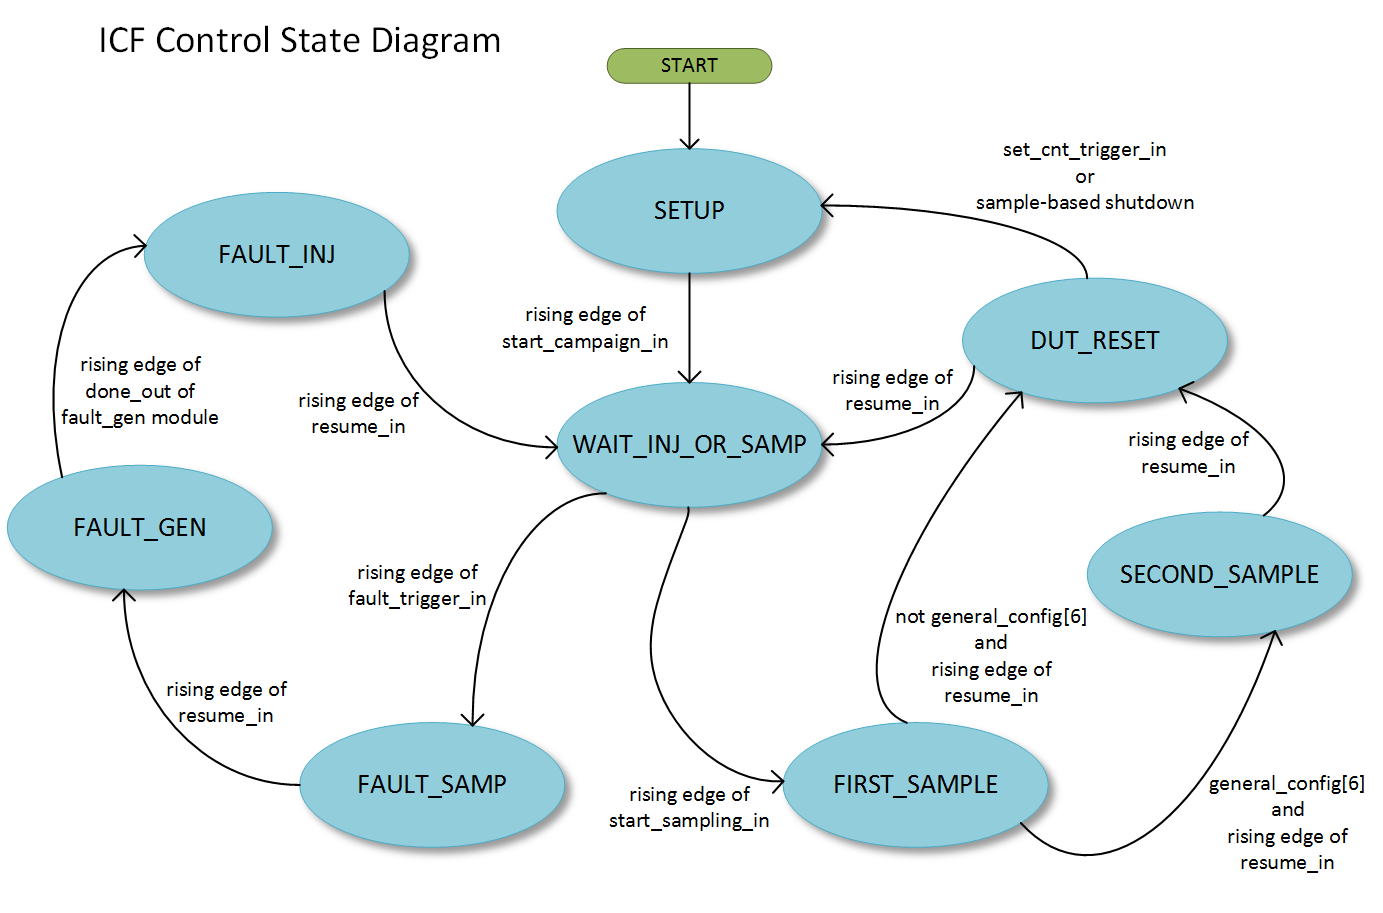
\includegraphics[width=0.7\linewidth]{../../technical_diags/f19_icf_master_fsm}
	\caption{ICF Control State Diagram}
	\label{fig:ic fmaster fsm}
\end{figure}

A description of each state are listed below.
\begin{itemize}
	\item SETUP: MISST registers are configured with desired values by user.
	\item WAIT\_INJ\_OR\_SAMP: DUT runs while MISST waits for the injection and the sampling timers to timeout. 
	\item FIRST\_SAMPLE: Retrieves the first sample. Value based shutdown is also evaluated here (see section \ref{ss samping-based shutdown} for more information).
	\item SECOND\_SAMPLE: Retrieves the second sample if two samples will be taken.
	\item DUT\_RESET: DUT is reseted in preparation for a new run with a different group of faults.
	\item FAULT\_SAMP: Sample the fault location.
	\item FAULT\_GEN: Generate a new fault and calculate corrupted data to inject. This process mainly takes place in the fault\_gen module.Refer to section \ref{ss fault generation} for high level description of fault generation. Refer to section \ref{ss fault gen module} for information on fault\_gen module.
	\item FAULT\_INJ: Injecting fault into target DUT.
\end{itemize}

\begin{center}
	\begin{longtable}{|c|p{11cm}|}
		\caption{ICF Port Descriptions}
		\label{table:icf port desc}\\
		\hline 
		Port Name & Description \\ 
		\hline 
		\endfirsthead
		\caption{ICF Port Description Continued.}\\
		\hline
		Port Name & Description\\
		\endhead
		\hline
		start\_campaign\_in & A rising edge starts a fault injection campaign.\\
		\hline     
		resume\_in & A rising edge signals state transition after an injection or sampling.\\              
		\hline
		alu\_data\_in [31:0] & Output from ALU module.\\       
		\hline
		alu\_range\_vio\_in & High if ALU experiences a range violation on a non-random operation (see Table \ref{table:alu port desc}).\\ 
		\hline
		alu\_rand\_range\_vio\_in & High if ALU experiences a range violation on a random operation (see Table \ref{table:alu port desc}).\\ 
		\hline
		reset\_in & Resets registers and ICF state.\\            
		\hline
		fault\_trigger\_in & A rising edge initiates a fault injection.\\      
		\hline
		sampling\_trigger\_in & A rising edge initiates sampling a single address on DUT. The data sampled is sent to user.\\
		\hline
		set\_cnt\_trigger\_in & A rising edge signals that the maximum number of sets has been met and to end the current fault injection campaign.\\   
		\hline
		clk\_in & Clock input.\\                 
		\hline
		samp\_inj\_start\_out & Rising edge initiates data sampling without sending data sampled to user. Kept high during sampling and cleared on rising edge of resume\_in. This is used for reading data at injection location.\\    
		\hline
		sample\_start\_out & Rising edge initiates data sampling to send data to user. Kept high during sampling and cleared on rising edge of resume\_in.\\   
		\hline
		inj\_start\_out & Rising edge initiates data injection using current fault parameters. Kept high during sampling and cleared on rising edge of resume\_in. This is used for reading data at injection location.\\           
		\hline
		data\_to\_regs\_out [31:0] & Data bus to register control and memory interconnect. Data headed to register control module will be injected into DUT during fault injection. Data headed to memory\_interconnect will be written to a Control Unit register.\\  
		\hline
		addr\_to\_regs\_out [31:0] & Address bus to register control and memory interconnect. Addresses sent to memory interconnect only use least significant byte and represents address of register. Addresses sent to register control represent an address in the DUT for injection or sampling.\\     
		\hline
		write\_data\_out & A write enable on rising edge for memory interconnect.\\         
		\hline
		fp\_wr\_out & A write enable on rising edge for Fault Parameter module.\\             
		\hline
		fp\_wr\_en\_out & An active high chip enable for Fault Parameter module.\\           
		\hline
		mux0\_sel\_out & Output to mutliplexer. If low, alu\_op\_out of Fault Parameter module outputs to func\_sel of the ALU. If set, func\_sel is connected to ALU-Fault Parameter bus. This bus can be driven by mux1\_data\_out if mux1\_sel\_out is set.\\          
		\hline
		alu\_oprnd\_sel\_out & Drives oprnd\_sel input of the ALU (see Table \ref{table:alu port desc}).\\       
		\hline
		mux1\_data\_out [31:0] & Data input for mux1(see Figure \ref{fig:core system interconnects}).\\      
		\hline
		mux1\_sel\_out & Drives selection input of mux1 (see Figure \ref{fig:core system interconnects}). When low, the ALU output op\_res drives the ALU-Fault Parameters bus. When high, mux1\_sel\_out drives the ALU-Fault Parameters bus.\\          
		\hline
		reset\_fault\_cnt\_out & Resets fault timer after a successful fault injection.\\   
		\hline
		reset\_sampling\_cnt\_out & Resets sampling timer after a successful sampling.\\ 
		\hline
		reset\_set\_cnt\_out & Resets set counter after a timeout, but before MISST enters setup mode.\\     
		\hline
		dut\_clk\_disable\_out & If high, disables DUT clock input to fault and sampling timers.\\    
		\hline
		campaign\_done\_out & Rising edge signals end of injection campaign.\\
		\hline      
	\end{longtable} 
\end{center}

\clearpage
%DONE
\subsection{The fault\_gen Module}
\label{ss fault gen module}

This module implements the logic described in section \ref{ss fault generation}. The module is implemented as three cycle counters in series and the first cycle counter in the chain being incremented for every generation request. Initializations are started when a level's associated timer timeouts. Updates are started when a level's associated cycle counter increments. 

\begin{center}
	\begin{longtable}{|c|p{11cm}|}
		\caption{fault\_gen Port Descriptions}
		\label{table:fault gen port desc}\\
		\hline 
		Port Name & Description \\ 
		\hline 
		\endhead
		gen\_request\_in & Initiates fault generation on rising edge.\\
		\hline
		reset\_in & Resets counters and registers on rising edge.\\     
		\hline
		clk\_in & Clock input.\\
		\hline
		rand\_range\_vio\_in & Connected from rand\_range\_vio output of ALU (see Table \ref{table:alu port desc}).\\
		\hline
		lvl2\_cyc\_len\_in [31:0] & Cycle length of level 2.\\
		\hline
		lvl1\_cyc\_len\_in [31:0] & Cycle length of level 1.\\
		\hline
		lvl0\_cyc\_len\_in [31:0] & Cycle length of level 0.\\
		\hline
		lvl2\_addr\_in [7:0] & Level 2 fault parameter name address (see section \ref{sec fp addr scheme}).\\
		\hline
		lvl1\_addr\_in [7:0] & Level 1 fault parameter name address (see section \ref{sec fp addr scheme}).\\
		\hline
		lvl0\_addr\_in [7:0] & Level 0 fault parameter name address (see section \ref{sec fp addr scheme}).\\
		\hline
		done\_out & Rising edge signals to ICF that fault generation is complete.\\
		\hline
		addr\_out [7:0] & Current fault parameter being updated.\\
		\hline
		w\_fp\_out &  Connected to write enable for Fault Parameter module.\\
		\hline
		wen\_fp\_out & Connected to chip enable for Fault Parameter module.\\
		\hline
		init\_on\_out & Set during an initialization operation. Cleared when operation is complete.\\ 
		\hline
		mux\_sel\_out [1:0] & Level being initialized. Outputs 0b00 (level 1), 0b01 (level 2), 0b10 (level 3), and 0b11 (nothing selected) sequentially as each level is updated.\\
		\hline
	\end{longtable}
\end{center}

%DONE
\section{Fault Timer, Sampling Timer, and Set Counter}
\label{s fault, samp, set timers}

During a fault campaign, the Control Unit responds to the timeouts of the three timers shown in Figure \ref{fig:control unit design}. Module cyc\_cnt0 counts the number of DUT clock cycles until a fault injection, and is reset by the ICF after fault injection is completed. Module cyc\_cnt1 counts the number of DUT clock cycles until sampling, and is reset by the ICF after sampling is completed. Module cyc\_cnt3 counts the number of sets completed so far. When this timer reaches its maximum value, the fault campaign is over. Whenever any of these counters timeout, the ICF takes the appropriate actions to execute the timer's associated action.

All three modules are instances of the cycle counter module. Refer to section \ref{ss cyc cnt} for more information on the cycle counter. 

%=====================================================================
%DONE
\chapter{Adapter Module}
\label{c adapter module}

The main purpose of the Adapter module is to provide an interface for the MISST core to communicate externally with a DUT or an intermediary module. In the case of the Original Implementation, for example, the Adapter module consists of an AXI slave module controlled by a Cortex processor. It is the user's responsibility to implement this module for their specific DUT.

For any implementation, the Adapter module is required to have certain ports and functional requirements. The required ports are listed in Table \ref{table:adapter required ports}. Using these ports, the adapter module can fill in the required bit-fields for the required register sys\_status. The bit-fields of sys\_status are shown in Table \ref{table:sys_status bit fields}. The reasoning for requiring sys\_status is that the adapter class needs to be aware of MISST high level behavior to properly coordinate traffic between the PC, MISST, and target DUT. For instance, the Adapter module needs to be aware if MISST is configured to send one or two samples to the user.

\begin{table}[h]
	\centering
	\caption{Required Adapter Ports}
	\begin{tabular}{|c|c|p{12cm}|}
		\hline 
		Port Name & I/O & Description \\ 
		\hline 
		data\_in & input & Data from MISST core. \\ 
		\hline 
		addr\_in & input & Destination address of incoming data. \\ 
		\hline 
		read\_in & input & Writes incoming data at incoming address on rising edge. \\ 
		\hline 
		campaign\_in & input & A high value signals system executing fault campaign. \\ 
		\hline 
		is\_sampling\_in & input & A high value indicates system during sampling process. \\ 
		\hline 
		is\_inj\_in & input & A high value indicates system during injection process. \\ 
		\hline
		samp\_inj\_in & input & A high value indicates that the value at the injection location is being read for corruption and injection. \\
		\hline 
		data\_out & output & Data to MISST core. \\ 
		\hline 
		addr\_out & output & Destination address of outgoing data to MISST. \\ 
		\hline 
		write\_out & output & Rising edge signals write enable for outgoing data at outgoing address to the Control Unit. \\ 
		\hline 
	\end{tabular} 
	\label{table:adapter required ports}
\end{table}

\begin{table}[ht]
	\centering
	\caption{Register sys\_status Bit Fields}
	\begin{tabular}{|c|p{0.75\textwidth}|}
		\hline 
		Bit Position & Description \\ 
		\hline
		0 & Set if campaign\_in port is high, low otherwise.\\
		\hline
		1 & Set if is\_sampling\_in port is high, low otherwise.\\
		\hline
		2 & Set if samp\_inj\_in port is high, low otherwise.\\
		\hline
		3 & Set if is\_inj\_in port is high, low otherwise.\\
		\hline
		4 & Set if DUT must be reset. Clear after DUT operation has been performed and MISST is signaled to continue.\\
		\hline
		5 & Set if MISST is configured to sample two locations, clear otherwise. This value should be assigned when the Adapter module receives a write to general\_config[6] (see Table \ref{tab:register summary}).\\
		\hline
		6 & Set if MISST is in setup mode, clear otherwise.\\
		\hline
	\end{tabular} 
\label{table:sys_status bit fields}
\end{table}

%=====================================================================
%DONE
\chapter{Original Implementation Details}
\label{c original imp details}

In this chapter we will primarily focus on the Adapter module implementation on the PYNQ board because the MISST system core does not change between implementations. For the original implementation, the adapter module includes the AXI slave interface, the Cortex hard processor, and a bridge from Xilinx IP library. The relevant ones are AXI AHBLite Bridge and the AXI APB Bridge. The IP library doesn't have an AXI to JTAG Bridge, but it does include a JTAG to AXI Master Bridge.   

%DONE
\section{Serial Communication}
The only way to access the UART port for PC serial communication is through the Cortex-A9 processor. The UART from the PYNQ board arrives at 115200 baud. If the MISST is implemented on a development board whose FPGA was direct access to a serial port, two design approaches could be:
\begin{itemize}
	\item Use adapter module as an interface between MISST system core and the PC.
	\item Include a soft processor in the adapter module to process communication between board elements and a PC.
\end{itemize}


\section{Role of Cortex Processor}
 The Cortex processor receives user input and sends data to MISST via AXI-Lite protocol to the AXI slave interface. The processor can read and write from/to the AXI slave interface, but the MISST system can't send data directly to the Cortex. The only way MISST can notify the processor of anything is via a single wire connection that triggers an interrupt on the processor (this is implemented as an output pin on the AXI slave). 
 
 MISST triggers an interrupt whenever it has to sample data from the DUT or inject a fault into the DUT. The processor evaluates what to do based on the value of the sys\_status register at the time of the interrupt. Figure \ref{fig:processorinterrupttaskstate} outlines how the processor keeps track of tasks. 
 \begin{itemize}
 	\item WAITING\_FOR\_INTT: Processor is waiting for interrupt.
 	\item SAMPLE\_N\_SEND: Processor reads from the DUT's memory and sends data to MISST and user through UART.
 	\item DUT\_RESET: Processor resets and then restarts DUT. Shortly after restarting DUT, processor writes data to sampling register to resume fault campaign.\\
 	\item SAMPLE\_INJ: Processor reads from DUT's memory and only sends sample data to MISST.\\
 	\item INJECT: Processor reads dut\_inj\_addr and dut\_data\_out registers, and writes dut\_data\_out data at address dut\_inj\_addr in DUT memory.
 \end{itemize} 

\begin{figure}[h]
	\centering
	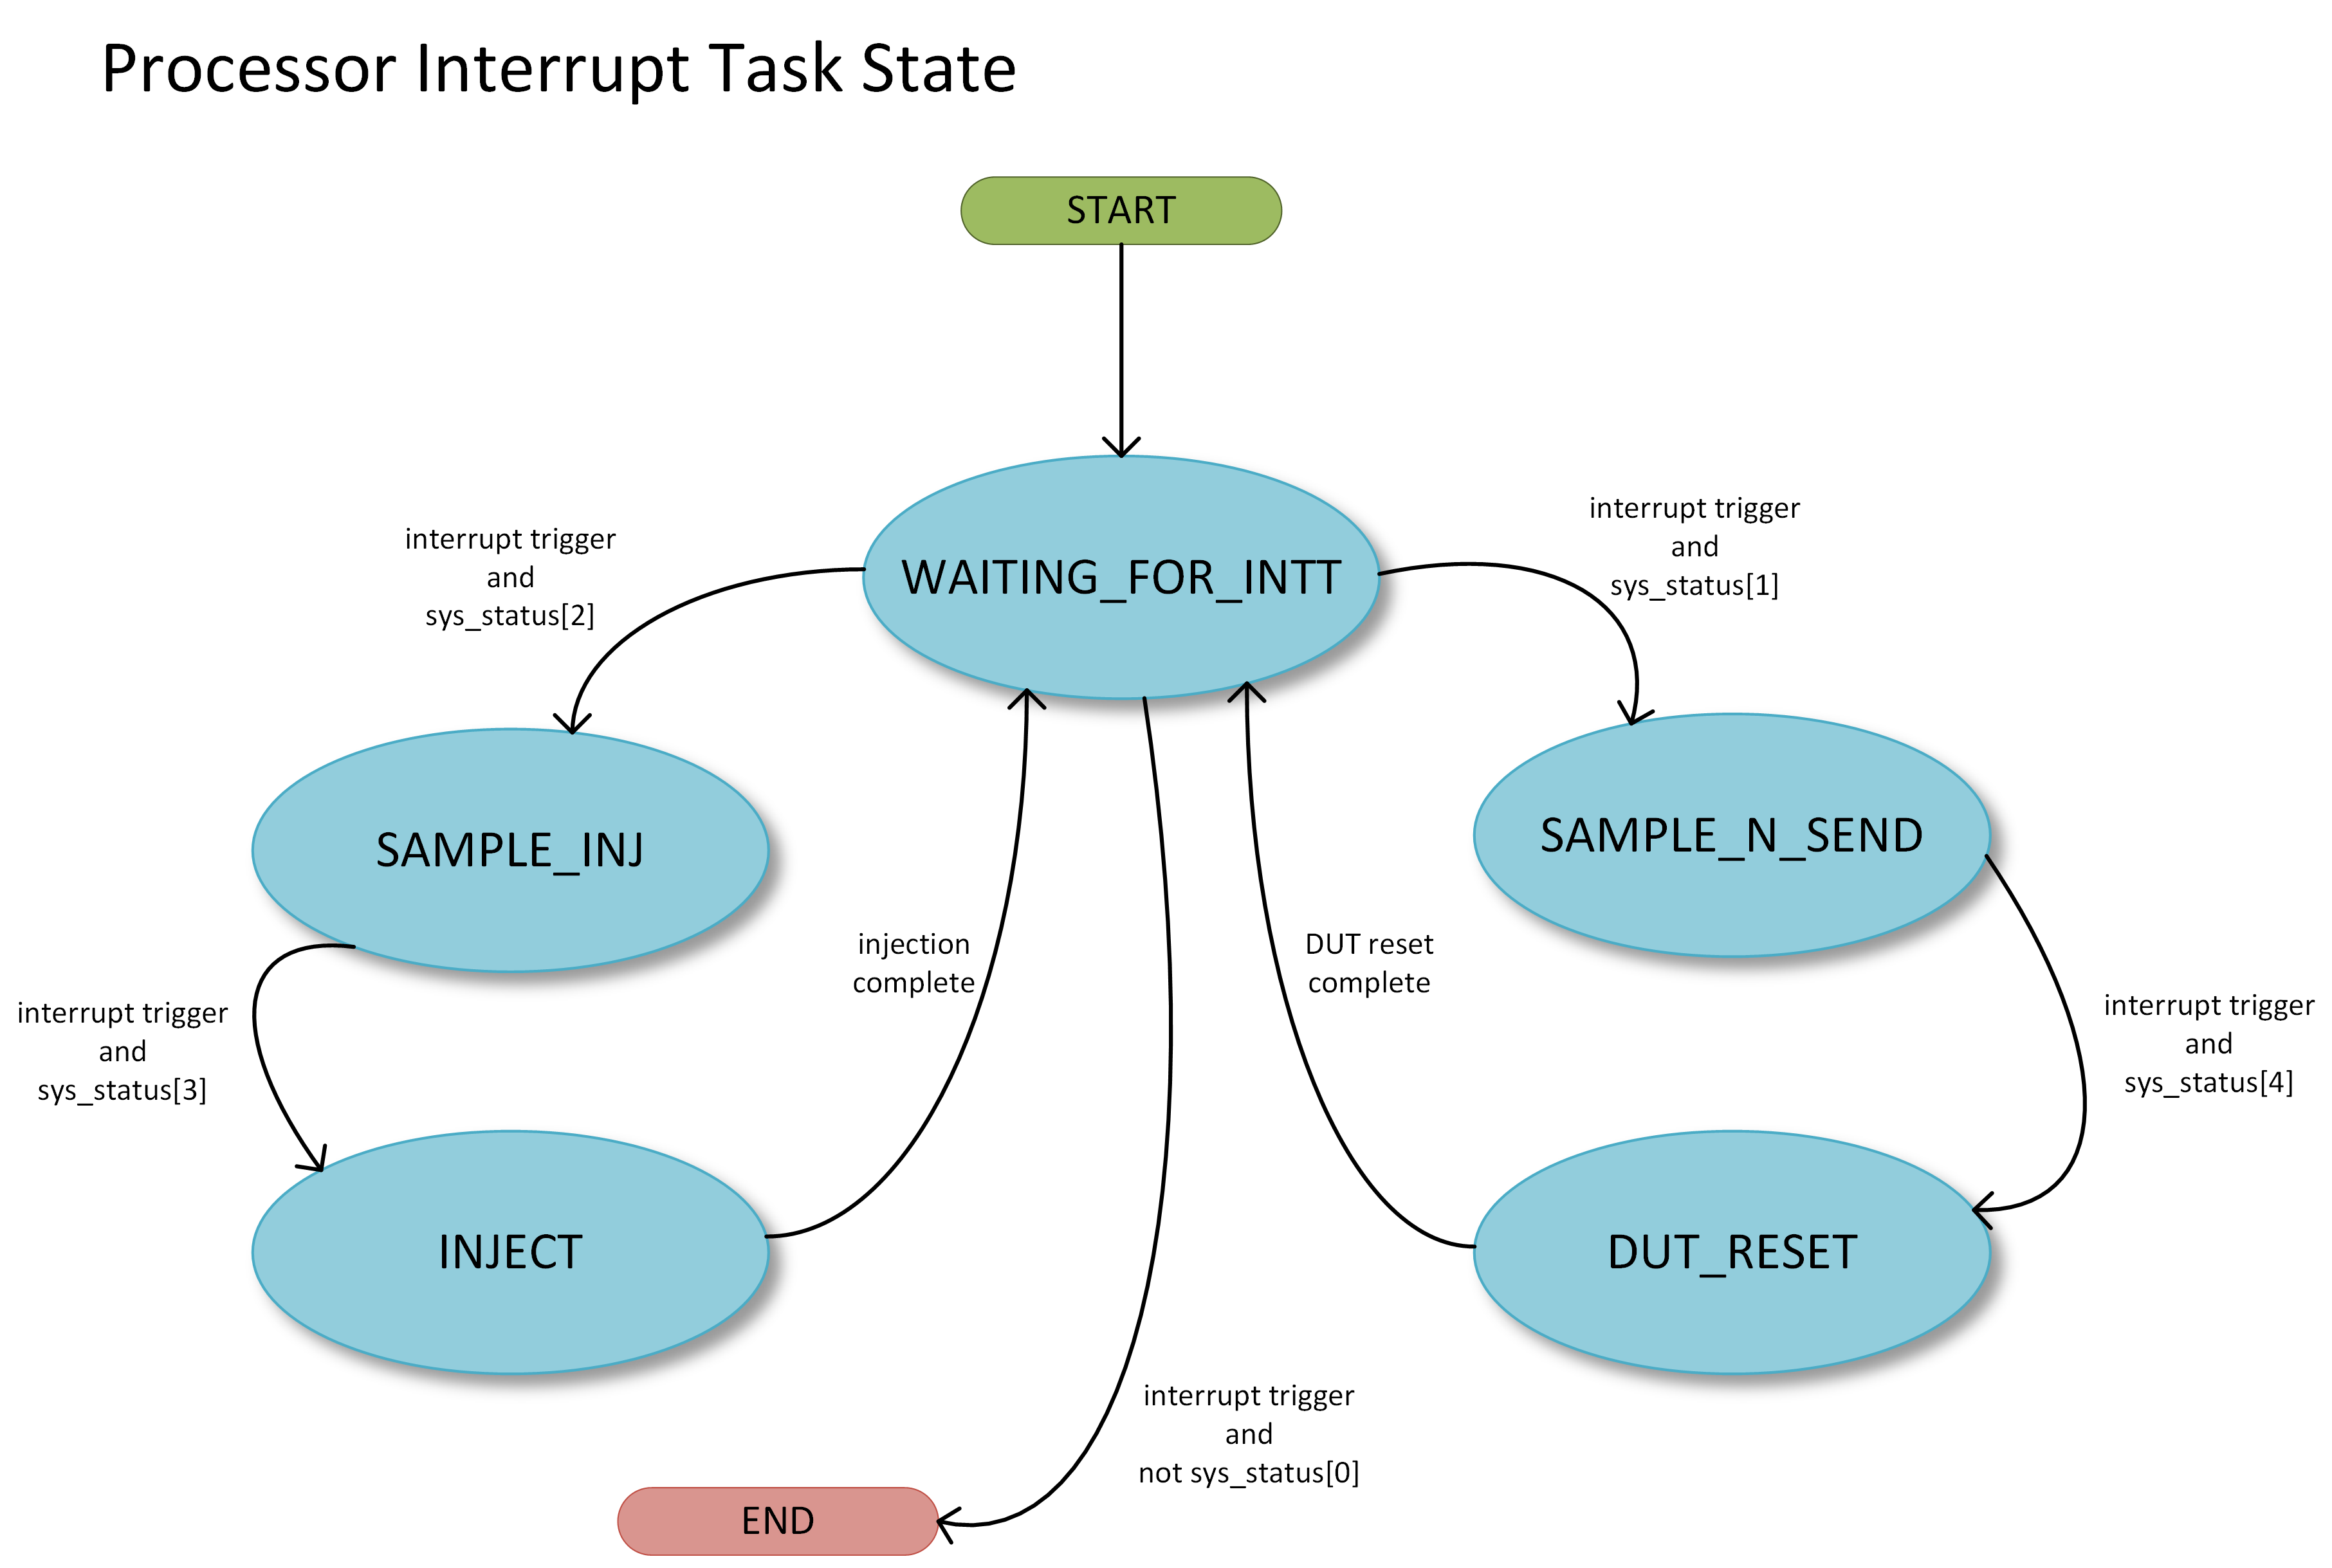
\includegraphics[width=0.8\linewidth]{../../technical_diags/f17_processor_interrupt_task_state}
	\caption{Processor Interrupt Task States}
	\label{fig:processorinterrupttaskstate}
\end{figure}

\clearpage
%DONE
\section{AXI Slave Interface}
\label{s axi slave interface}

During setup, the user is simply writing data to registers in MISST core. In order to write to MISST registers, the processor first writes the data to the AXI slave's w\_data register. Then the processor writes the write address to w\_reg\_addr register. The write is automatically executed upon a write to the w\_reg\_addr register. Table \ref{table:axi slave int regs} lists registers implemented on the AXI slave interface. All AXI slave interface registers are four bytes wide, but not all registers use four bytes.

\begin{table}[h]
	\centering
	\caption{AXI Slave Interface Registers}
	\begin{tabular}{|c|c|p{0.75\textwidth}|}
		\hline 
		Address & Register Name & Description \\ 
		\hline
		0x0C & sys\_status & Required register. Used by processor to choose correct course of action. See Table \ref{tab:register summary}.\\
		\hline
		0xC0 & dut\_sample\_addr & Sampling address.\\
		\hline
		0xC1 & dut\_inj\_addr & Injection address.\\
		\hline
		0xC2 & dut\_data\_out & Data to write to DUT. Only used during fault injection.\\
		\hline
		0xC3 & w\_reg\_addr & Write address of register in MISST. Writing to this register starts writing transaction to selected MISST register. Only uses least significant byte since register addresses are a byte long.\\
		\hline
		0xC4 & w\_data & Write data.\\
		\hline
	\end{tabular} 
	\label{table:axi slave int regs}
\end{table}

The AXI slave interface is also responsible for asserting the interrupt input of the processor. The AXI slave sets the interrupt pin if is\_sampling\_in, samp\_inj\_in, or is\_inj\_in are high. Most importantly, the AXI slave interface must conform to the Adapter-Core interface. Table \ref{table:axi slave ports} describes the AXI slave's ports and points out which ones are required by the Adapter-Core interface. 

\begin{table}[h]
	\centering
	\caption{AXI Slave Interface Port Descriptions}
	\begin{tabular}{|c|p{0.75\textwidth}|}
		\hline 
		Port Name & Description \\ 
		\hline
		data\_in [31:0] & Input data bus. Part of the Adapter-Core interface.\\
		\hline
		addr\_in [7:0] & Input address bus. Part of the Adapter-Core interface.\\
		\hline
		read\_in & Reads address and bus lines on rising edge.\\
		\hline
		is\_sampling\_in & A high value represents that MISST is in the process of sampling. The data sampled will be sent to the user. Part of the Adapter-Core interface.\\
		\hline
		samp\_inj\_in & A high value represents that MISST is in the process of sampling. The data sampled will not be sent to the user. Part of the Adapter-Core interface.\\  
		\hline
		is\_inj\_in & A high value represents that MISST is in the process of fault injection. Part of the Adapter-Core interface.\\ 
		\hline
		campaign\_in & A high value represents that MISST is running a fault campaign. Part of the Adapter-Core interface.\\
		\hline
		S\_AXI & Name for all signals of the AXI-LITE protocol. The processor sends data and reads data to/from here.\\
		\hline
		pause\_intt\_out & Connected to the processor's interrupt inputs. Referred to as the interrupt pin.\\
		\hline
		reset\_out & Resets MISST core.\\
		\hline
		data\_out [31:0] & Data bus to Control Unit. Part of the Adapter-Core interface.\\ 
		\hline
		addr\_out [7:0] & Address bus to Control Unit. Part of the Adapter-Core interface.\\
		\hline
		write\_out & Write enable for data sent to Control Unit. Part of the Adapter-Core interface.\\
		\hline
	\end{tabular} 
	\label{table:axi slave ports}
\end{table}

\FloatBarrier

The Adapter-Core interface provides rules on how the MISST core and the Adapter module exchange data. The Adapter-Core interface requires the ports with the following functionality:
\begin{itemize}
	\item A pair of data bus, address bus, and enable signals for read and write with the Control Unit. The read or write operation is executed on a rising edge of the enable signal.
	\item A signal that goes high during the sampling process and clears when sampling data has been received. Sampled data is sent to the user. \\
	\item A signal that goes high during the sampling process and clears when sampling data has been received. Sampled data is not sent to the user.\\
	\item A signal that goes high during the injection process and clears when fault injection process is complete.\\
\end{itemize}

%=====================================================================
\begin{thebibliography}{2}
	\bibitem{pynq board manual}PYNQ-Z1 Board Reference Manual. (2018). [ebook] Pullman. Available at: https://reference.digilentinc.com/\_media/reference/programmable-logic/pynq-z1/pynq-rm.pdf [Accessed 24 Feb. 2018].
	
	\bibitem{noise gen site} T. Storey. "Pseudo Random Number Generator with Linear Feedback Shift Registers (VHDL)." Internet: https://eewiki.net/pages/viewpage.action?pageId=10125438, Sept. 8, 2017 [March 1, 2018].
	
\end{thebibliography}

	
\end{document}